\chapter{RD53A}

Il progetto di RD53A è stato approvato nell'autunno del 2015, dopo la revisione da parte delle collaborazioni ATLAS, CMS e RD53A. Nel 2016 è iniziata la progettazione, con questo nuovo chip si vuole dimostrare la possibilità di utilizzare tecnologia CMOS  in 65 nm per l'aggiornamento in vista della fase ad alta luminosità di ATLAS e CMS, e quindi la tolleranza al danneggiamento da radiazioni, soglie di lavoro basse e stabili nel tempo, capacità di gestire un alto flusso di particelle incidenti e l'utilizzo di trigger veloci.

\section{Organizzazione del chip} 
RD53A non deve essere inteso come il prodotto finale, infatti possiede molte modifiche di design utili solo in una prima fase di test, ad esempio al suo interno sono presenti tre diversi front end (FE), già questo causa una non uniformità del chip. 
Questo chip è la base di partenza per arrivare al progetto finale, in cui sarà scelto uno dei front end e sarà utilizzato uniformemente su tutta la matrice di pixel. In RD53A la matrice di pixel ha 400 colonne e 192 righe, nel progetto finale si avrà un aumento del numero di pixel, infatti il sistema di alimentazione e di contropolarizzazione dei pixel è progettato per un numero di righe massimo pari a 384, figura \ref{RD53ALayout}.
\begin{figure}
\centering
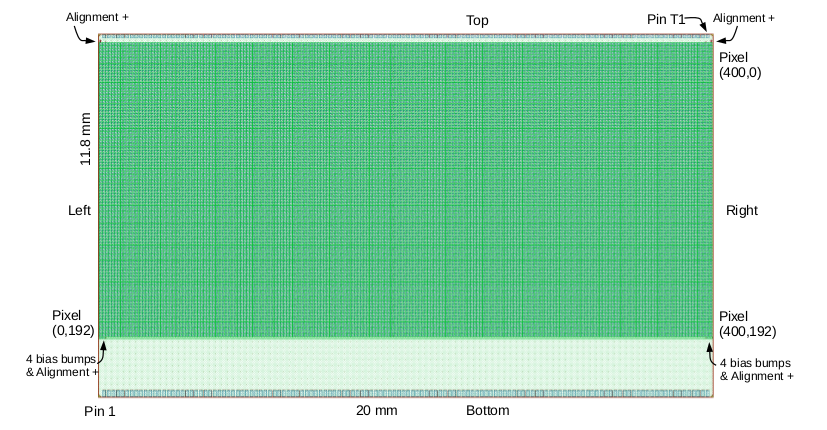
\includegraphics[scale=.4]{Immagini/RD53ALayout}
\caption{RD53A layout. Il chip è largo 20mm per 400 pixel e l'altezza è 11.8 mm per 192 pixel.}
\label{RD53ALayout}
\end{figure}

L'area del chip che sarà bondata al sensore è posta nella parte alta ed è organizzata secondo una matrice di 192 x 400 pixel di area 50 $\mu$m x 50 $\mu$m, sopra a questa è presente una fila di pad utilizzate per debug, questa sarà eliminata nella versione finale. La parte di circuito necessaria per configurare monitorare e leggere il chip è posta nella parte bassa, sotto cui è posta una fila di pad per i wire-bond. 
La matrice di pixel è organizzata in \textit{cores} di 8 x 8 pixel, all'interno i 64 front end sono disposti in gruppi di 4, chiamati isole analogiche, figura \ref{AnalogIsland}. 
Queste isole sono circondate da un "mare" digitale, il circuito introno ad ogni isola è differente. 
\begin{figure}
\centering
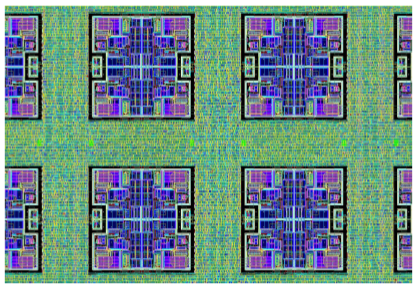
\includegraphics[scale=.5]{Immagini/AnalogIsland}
\caption{Immagine al microscopio della disposizionein gruppi di 4 dei front end.}
\label{AnalogIsland}
\end{figure} 
Nelle parti più esterne del chip tutti i blocchi analogici sono raggruppati in macro blocchi chiamati Analog Chip Bottom (ACB). Il blocco ACB è circondato dal blocco Digital Chip Bottom (DCB) che implementa la logica digitale per Input, Output e configurazione.
\section{Front End}
Come detto in precedenza RD53A non è il chip finale, ma un prototipo, al cui interno sono presenti tre differenti Front End per la parte analogica. Si tratta di tre differenti progetti e sono indicati con i nomi: Sincrono, Lineare e Differenziale, vedi figura \ref{FrontEnd}. 
Questi tre circuiti sono stati progettati da tre differenti gruppi e tra di loro ci sono importanti differenze. Il FE Sincrono sfrutta un sistema di auto-zeroing della linea di base, campionando periodicamente la linea di base invece di aggiustare la soglia pixel per pixel. 
Il Lineare implementa un amplificatore lineare all'ingesso del comparatore, il cui compito è confrontare il segnale con una certa soglia. 
Nel Differenziale è presente uno stadio di guadagno differenziale  all'ingresso del discriminatore e sbilanciando i due canali implementa la soglia.
Le caratteristiche comuni sono le piazzole per i bump-bond e il layout. Inoltre è comune anche la rete di polarizzazione ed il circuito per iniettare segnali di calibrazione, in modo da poter comparare direttamente le prestazioni. 
I tre FE condividono l'area del sensore e dato che la matrice è larga 400 pixel ed è suddivisa in core da 8 $\times$ 8 pixel, dunque non è possibile avere una egual area per i tre tipi di FE. Due avranno 17 core e uno solo ne avrà 16. I FE Lineare e Differenziale sono stati posti accanto in quanto hanno funzionalità simili e metterli vicino consente di avere un'area maggiore con una risposta il più uniforme possibile. 
\begin{figure}
\centering
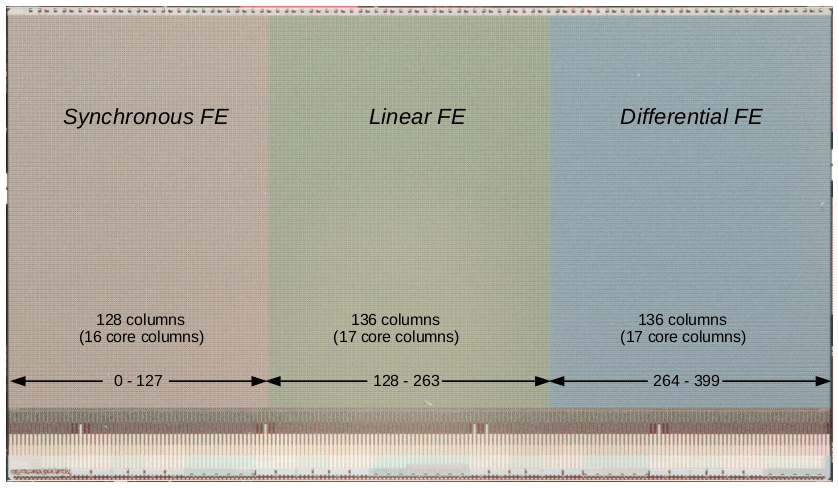
\includegraphics[scale=.3]{Immagini/FrontEnd}
\caption{Disposizione dei tre differenti Front End rispetto alla matrice di pixel 192 x 400.}
\label{FrontEnd}
\end{figure}

Di seguito è riportata una breve descrizione del funzionamento di ciascuno dei tre Front End:
\begin{itemize}

\begin{figure}
\centering
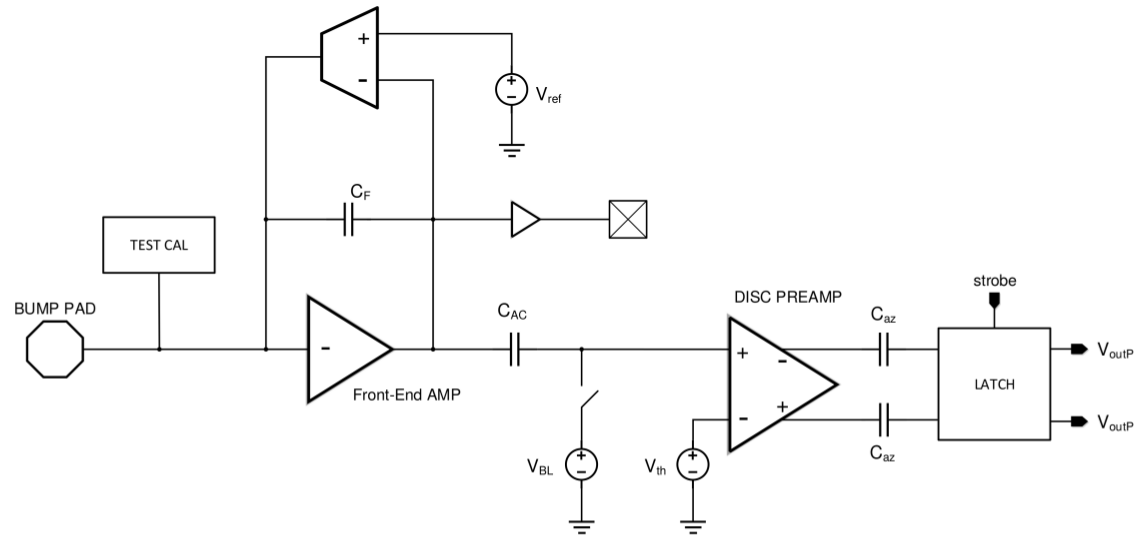
\includegraphics[scale=.3]{Immagini/SchemaSincrono}
\caption{Schematico del front end Sincrono.}
\label{SchemaSincrono}
\end{figure}
\item \textbf{Sincrono}. Uno schema a blocchi del front end Sincrono è riportato in figura \ref{SchemaSincrono}. 
Questo front end consta di un CSA a stadio singolo con Krummenacher feedback accoppiato in AC ad un discriminatore sincrono formato da un amplificatore differenziale e un latch di feedback positivo. 
Il Krummenacher feedback è progettato in modo da fornire sia la compensazione alla corrente dispersa dal sensore sia la corrente di scarica per la capacità presente nell'anello di reazione. Maggiore è la corrente più veloce il segnale del pre amplificatore tornerà alla baseline. 
Consideriamo come riferimento che, una carica di di 10k$e^{-}$, che produce 10 nA di corrente e un segnale che dura 400 ns è ridotta circa ad un segnale di 40 nA corrente per una durata di 100 ns.  
Al fine di avere due differenti valori di guadagno sono incluse due capacità, rispettivamente di 2.5 fF e 4 fF. 
A causa di piccole differenze, che sono rilevanti a scale di 65 nm, si hanno fluttuazioni abbastanza ampie della baseline in uscita dal primo stadio (dell'ordine delle decine di millivolt) tra canali differenti. 
Per eliminare queste differenze si è reso necessario un accoppiamento in AC al dicriminatore. 
In ogni caso le differenze tra transistor si traducono in un offset della tensione in uscita dal discriminatore tra i vari pixel. 
Questo effetto normalmente è compensato con DAC usati localmente per regolazioni fini, invece, nel front end Sincrono l'offset è compensato attraverso un meccanismo di auto azzeramento. 
Ciò richiede l'acquisizione del livello di tensione della baseline ogni 100 $\mu$s o meno. Durante le collisioni, la differenza tra segnale e la baseline letta è inviato ad uno stadio che fa il confronto e genera il segnale di uscita del discriminatore.  

\begin{figure}
\centering
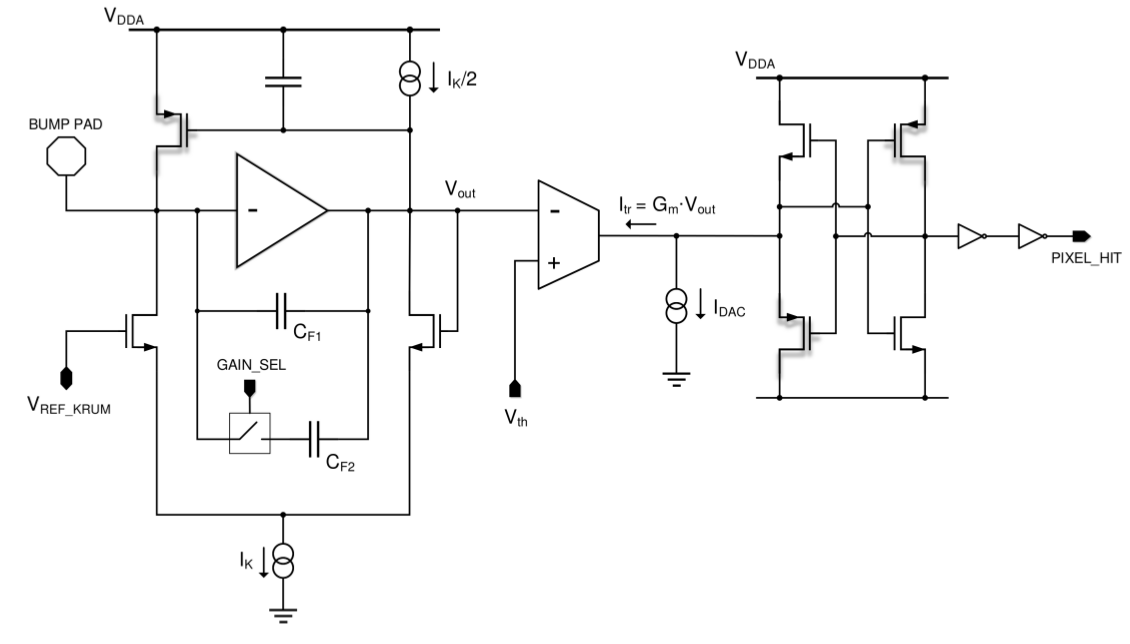
\includegraphics[scale=.3]{Immagini/SchemaLineare}
\caption{Schematico del front end Lineare.}
\label{SchemaLineare}
\end{figure}
\item \textbf{Lineare}. Il Front End lineare è mostrato in figura \ref{SchemaLineare}. Il circuito di lettura include un amplificatore di carica  (\textit{Charge Sensitive Amplifier}) con un Krummenacher feedback al fine di far fronte  dell'aumento di corrente di dispersione, indotte degli alti livelli di radiazione attesa. 
La scelta di un amplificatore a stadio singolo è stata dettata semplicemente dai limiti imposti sui consumi e lo spazio limitato disponibile. 
Il segnale ottenuto dal CSA è mandato ad un comparatore che, insieme al contatore ToT (\textit{Time over Threshold}), è utilizzato per fare la conversione a segnale digitale. 
Canale per canale gli aggiustamenti della tensione di soglia sono gestiti da un circuito locale basato su un binary weighted DAC a 4 bit che genera una corrente $\mathrm{I_{DAC}}$, fornendo una regolazione locale della soglia. 
Questo tipo di front end è stato ottimizzato per una carica massima corrispondete a 30000 elettroni con un consumo complessivo di circa 4 $\mu$A. 
Il CSA può essere utilizzato in regime di alto o basso guadagno andando a modificare il bit GAIN$\_$SEL, mentre la corrente di recupero $\mathrm{I_K}$/2 proveniente dal circuito di Krummenacher feedback può essere configurato tramite un DAC. 
In configurazione di alto guadagno per un segnale di carica pari a 30000 elettroni si ha un ToT di circa 400 ns che risulta in una corrente $\mathrm{I_K}$ di 25 nA. 
La risoluzione aspettata in configurazione di alto guadagno è di 15 mV/k$e^{-}$, mentre è di 7.5 mV/k$e^{-}$ con basso guadagno. 
Le prestazioni del preamplificatore di carica sono determinate principalmente dall'ingresso del CSA e la parte del circuito di feedback  con transistor PMOS. Nelle simulazioni il rumorein carica equivalente, per un rivelatore con capacità di 50 fF, è pari a 87 elettroni. 
Da simulazioni la dispersione della soglia dovrebbe passare da 380 elettroni a 35 elettroni dopo la messa a punto.

\begin{figure}
\centering
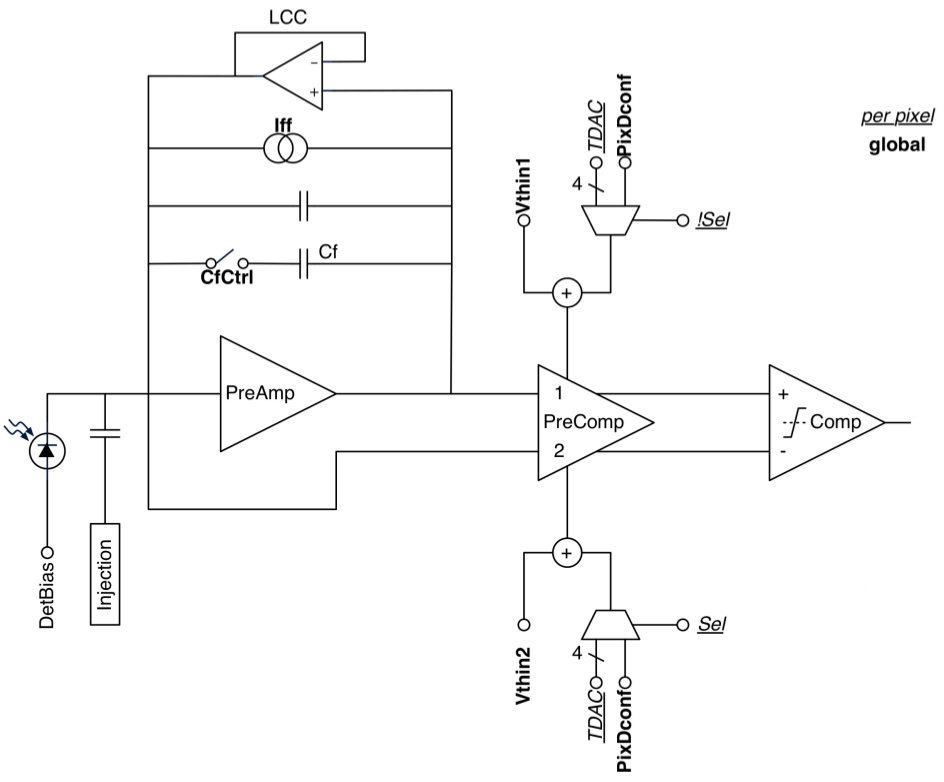
\includegraphics[scale=.3]{Immagini/SchemaDifferenziale}
\caption{Schematico del front end Differenziale.}
\label{SchemaDifferenziale}
\end{figure}
\item \textbf{Differenziale}. Il front end Differenziale è un circuito puramente analogico: non ha al suo interno latches, flip-flop o contatori. 
I valori di configurazione sono però forniti da un nucleo digitale, che dalla parte analogica riceve solo il segnale in uscita del comparatore. 
Naturalmente è necessaria la presenza di un ADC per la digitalizzazione del ToT ottenuto dal comparatore, anch'esso è implementato interamente nella parte digitale. 
Lo schema a blocchi del front end differenziale è riportato in figura \ref{SchemaDifferenziale}. 
Il preaplificator presente nel primo stadio ha un guadagno continuo regolabile andando a scegliere tra i due valori possibili di capacità presenti nell'anello di reazione. Questo feedback in corrente è impostato globalmente e non può essere regolato su ogni singolo pixel. 
Dalle misure sui prototipi è stato visto che la conseguente dispersione nei valori di ToT ha un livello accettabile senza necessità di una pre regolazione.  
In caso di assenza di segnale il feedback assicura che input e output del preamplificatore siano allo stesso potenzioale.
Nel secondo stadio il pre comparatore fornisce un guadagno aggiuntivo e agisce come soglia differenziale. 
La soglia globale può essere regolata tramite le tensioni VTH1 e VTH2. 
Localmente la soglia è modificata utilizzando un resistor ladder a 4 bit a livello in ciascuno dei due rami del pre comparatore. Oltre a i 4 bit c'è un quinto bit che seleziona quale dei due rami modificare. 
Dopo il pre comparatore si ha uno stadio con un comparatore la cui uscita è collegata alla regione digitale tramite porte logiche. 
Progettato per operare con una soglia di 500 elettroni, la parte analogica ha un consumo di 4$\mu$A/pixel , considerando una capacità di 50 fF e 10 nA di corrente dispersa.


\end{itemize}

\section{Alimentazione}
\begin{figure}
\centering
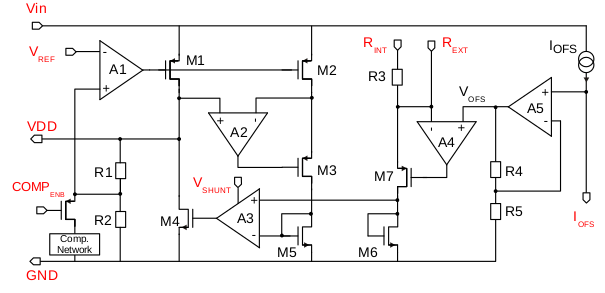
\includegraphics[scale=.6]{Immagini/SLDO_RD53A}
\caption{Regolatore LDO con Shunt (Shunt-LDO).}
\label{SLDO_RD53A}
\end{figure}
In RD53A l'alimentazione è gestita da due regolatori LDO con shunt, uno per la parte analogica ed uno per quella digitale. 
Rispetto al circuito di SLDO presentato in precedenza vi sono delle differenze, in particolare la tensione di offset è generata con un circuito diverso, lo schema del circuito di SLDO è riportato in  figura \ref{SLDO_RD53A}. 
I valori di Input e Output sono riportati nella seguente tabella:
\begin{center}
\begin{tiny}
\begin{tabular}{|c|c|c|c|c|l|}
\hline
\textbf{Pin} & \textbf{Tipologia} & \textbf{Minimo} & \textbf{Tipico} & \textbf{Massimo} & \textbf{Descrizione} \\ \hline

$\mathrm{V_{IN}}$ & Alimentazione & 1.4 V & & 2.0 V & Input di alimentazione esterna (in tensione)\\ \hline
 & Power & 0 A & 0.5 A & 2.0 A & Input di alimentazione esterna (in corrente)\\ \hline     
$\mathrm{V_{SHUNT}}$ & Alimentazione & 1.4 V & & 2.0 V & Tensione di alimentazione per il circuito di shunt\\ \hline
GND & Ground &  & &  & Terra locale e uscita della corrente di shunt\\ \hline
VDD & Alimentazione & 1.0 V & 1.2 V & 1.32 V & Tensione di uscita del regolatore\\ \hline
$\mathrm{V_{REF}}$ & Analogico & 500 mV & 600 mV & 660 mV & Tensione di riferimento (VDD=2$\mathrm{V_{REF}}$\\ \hline
$\mathrm{R_{INT}}$ & Analogico &  & $\mathrm{V_{IN}}$ &  & Enable resistenza interna R\\ \hline
$\mathrm{R_{EXT}}$ & Analogico & 300 $\Omega$ &  &  & Resistenza esterna collegata a $\mathrm{V_{IN}}$\\ \hline
$\mathrm{I_{OFS}}$ & Analogico &  & 200 k$\Omega$ &  & Resistenza esterna connessa a GND\\ \hline
$\mathrm{COMP_{ENB}}$ & Digitale &  & GND &  & Segnale per abilitare il circuito di compensazione\\ \hline
\end{tabular}
\end{tiny}
\end{center}

Infatti, è possibile applicare al terminale $\mathrm{I_{ofs}}$ una resistenza che con la sua caduta di tensione determina il valore di $\mathrm{V_{ofs}}$. 
Questa resistenza va saldata sulla Single Chip Card nell'apposito slot. Il valore di $\mathrm{I_{ofs}}$ è 2 $\mu$A, quindi:
\begin{equation}
\label{eq:Vofs}
\mathrm{V_{ofs} = 2 \mu A \cdot R_{iofs}}
\end{equation}
Questa tensione viene raddoppiata tramite l'azione dell'anello di reazione di A5, prima di essere mandata ad A4.
Riepilogando il comportamento della tensione in ingresso sarà:
\begin{equation}
\mathrm{V_{in}= 2 \cdot V_{iofs} + \dfrac{R3}{1000} \cdot I_{in}}
\end{equation}
Nelle misure che sono presentate nelle sezioni successive ogni volta che si parlerà di R3 e $V_{ofs}$ interni si farà riferimento ai seguenti valori:

\begin{center}
\begin{tabular}{lc}
\hline
$\mathrm{R3}$ & 600 $\Omega$ \\%misurata con il multimetro è 620
$\mathrm{R_{iofs}}$ & 250 k$\Omega$\\ 
\hline
\end{tabular}
\end{center}
Per quanto detto in precedenza, equazione \ref{eq:Vofs}, una $\mathrm{R_{iofs}}$ di 250 k$\Omega$ corrisponde ad una tensione di offset di circa 0.5 V. Perciò nell'andamento della tensione in ingresso, in funzione della corrente, ci aspettiamo un offset di circa 1 V.

Per quanto riguarda le tensioni di riferimento, come $\mathrm{V_{ref}}$, queste vengono generate all'interno del chip da un circuito dedicato in cui vengono utilizzati bandgap. Il valore di uscita dei bandgap è configurabile, di default ha un valore 16 che corrisponde circa a una tensione di 1.15 V. 
Questo valore varia leggermente da un chip all'altro, un esempio è riportato in figura \ref{bandgap_trimming}, dove sono riportati gli andamenti di $\mathrm{V_{ref}}$ al variare del valore di configurazione per differenti chip.

\begin{figure}
\centering
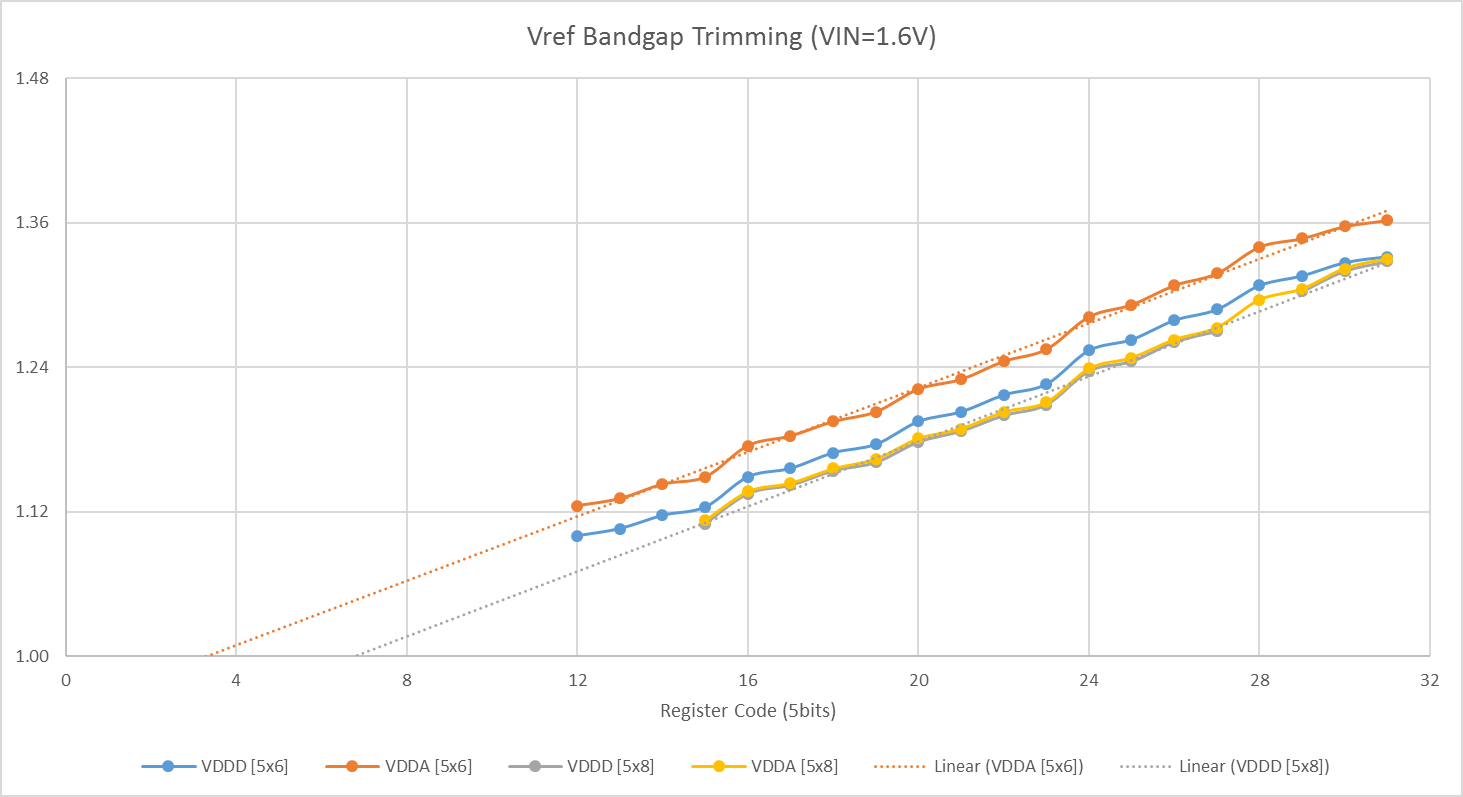
\includegraphics[scale=.5]{Immagini/bandgap_trimming}
\caption{Andamento della tensione di $\mathrm{V_{ref}}$ generata internamente, per due diversi chip, al variare del parametro di configurazione, il valore di default è 16.}
\label{bandgap_trimming}
\end{figure}

\section{Single Chip Card}
Analogamente a quanto visto per gli SLDO, per  testare i quali si fa uso di una PCB di test, per il chip RD53A è necessario l'utilizzo di una SCC (\textit{Single Chip Card}). 
Il chip è fissato al centro di questa scheda e attraverso wire bond è connesso ai vari elementi della scheda (pin di monitoraggio, molex di alimentazione, DisplayPort per la trasmissione/ricezione di dati, jumper per la configurazione, etc...). 
Il chip viene montato sulla scheda in un apposito spazio ai cui bordi arrivano le varie piste da connettere e sotto cui, al posto della vetronite, c'è uno spessore metallico con via termici in modo da permettere l'applicazione di un sistema refrigerante sulla parte posteriore della SCC. 
La presenza di un raffreddamento è necessaria nel momento in cui l'alimentazione è data utilizzando i due SLDO, la corrente non necessaria al chip viene dissipata sui due shunt che diventano punti molto caldi. 
Al fine di evitare danneggiamenti del chip e dell'eventuale sensore che vi può essere collegato il chip va raffreddato con l'utilizzo di dissipatori di calore. 

Dal momento che il chip è un prototipo è stata lasciata la possibilità di poter configurare l'alimentazione esternamente scegliendo tra tre diverse configurazioni e inoltre è possibile mantenere separate a livello di alimentazione la regione digitale e quella analogica\footnote{Nel chip finale gli ShuntLDO della parte digitale e analogica saranno in parallelo.}.
Le possibili configurazioni sono:

\begin{itemize}
\begin{figure}
\centering
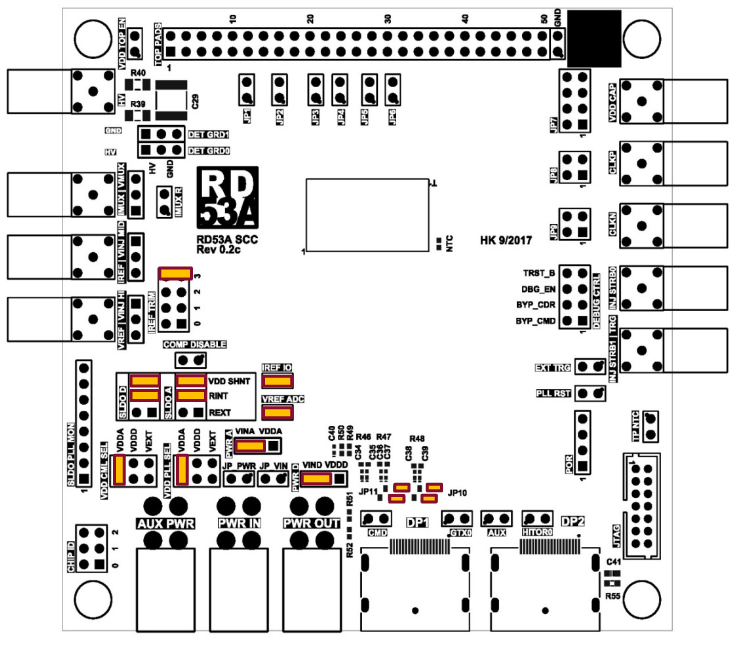
\includegraphics[scale=.3]{Immagini/SLDOmode}
\caption{Configurazione dei jumper per l'utilizzo di RD53A alimentato attraverso il circuito di ShuntLDO, sia per la regione analogica sia per quella digitale.}
\label{SLDOmode}
\end{figure}
\item Alimentazione del attraverso il circuito di ShuntLDO, in questo caso il generatore utilizzato sarà di corrente e sulla SCC card la configurazione dei jumper sarà quella riportata in figura \ref{SLDOmode}. 
Per operare con il chip in configurazione SLDO è necessario l'utilizzo di un sistema di raffreddamento per il chip. 
In normali condizioni di lavoro è sufficiente un dissipatore passivo, va però sottolineato che nella misura delle varie tensioni l'effetto di deriva termica non è trascurabile, dunque l'ideale sarebbe l'utilizzo di un sistema di raffreddamento attivo, con un buon contatto termico, che permetta di controllare le temperature.

\begin{figure}
\centering
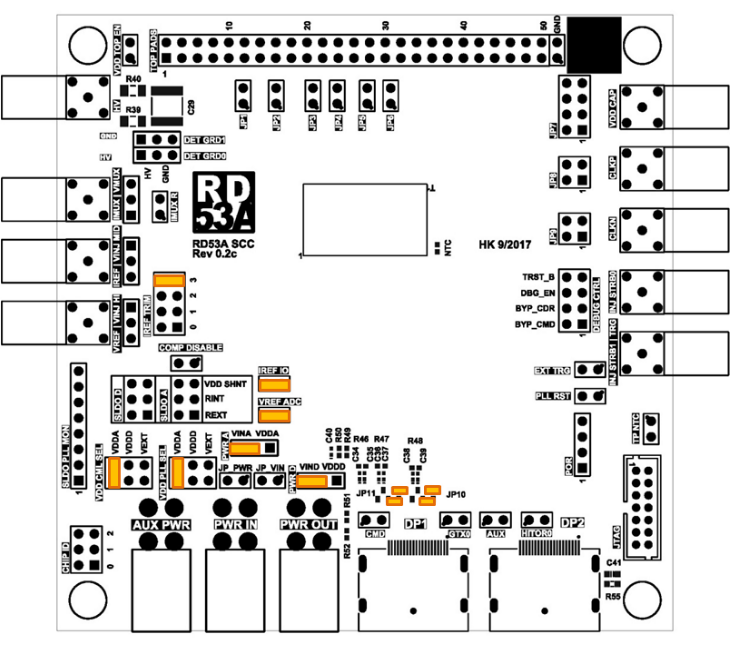
\includegraphics[scale=.3]{Immagini/LDOmodeDefault}
\caption{Configurazione dei jumper per l'utilizzo di RD53A alimentato dal regolatore LDO senza la parte di shunt.}
\label{LDOmode}
\end{figure}
\item Alimentazione senza Shunt, utilizzando solo il regolatore LDO. Questa configurazione necessita di una alimentazione in tensione, in questo caso sarà il generatore esterno a dover generare più o meno corrente al variare dei consumi del chip. L'utilizzo del solo regolatore permette di avere un consumo minimo in termini di potenza e dunque di operare con il chip senza il bisogno di un sistema di raffreddamento. In questo caso la configurazione dei jumper è quella riportata in figura \ref{LDOmode}.

\begin{figure}
\centering
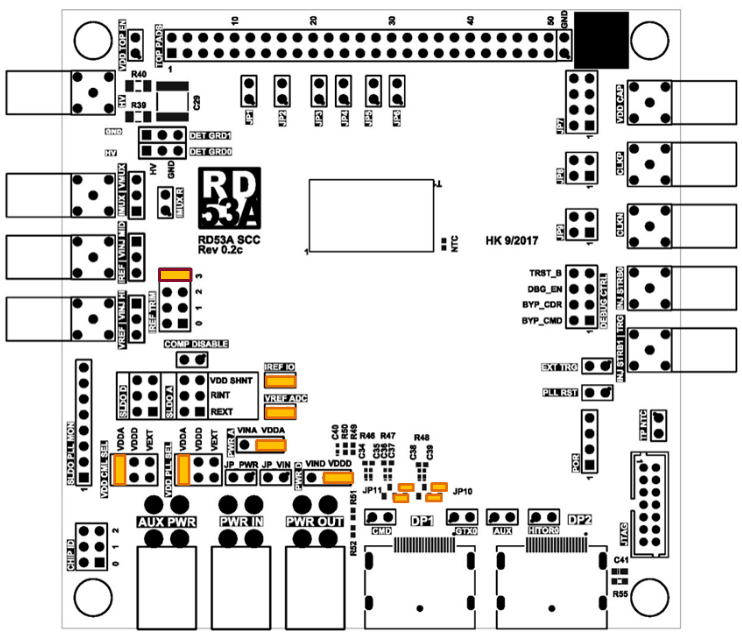
\includegraphics[scale=.3]{Immagini/DirectPowering}
\caption{Configurazione dei jumper per l'utilizzo di RD53A alimentato direttamente, escludendo il circuito di ShuntLDO.}
\label{DirectPowering}
\end{figure}
\item Alimentazione diretta. In questo caso il circuito con regolatore e shunt viene completamente escluso ed il chip è alimentato direttamente dal generatore di tensione. 
Questa configurazione è riportata in figura \ref{DirectPowering}, l'utilizzo dell'alimentazione diretta è delicato per varie ragioni, prima fra tutte il rischio di danneggiamento di RD53A. 
La presenza del regolatore LDO, anche privo di shunt, assicura che sbalzi di tensione all'ingresso dell'alimentazione non siano trasmessi al chip, inoltre il regolatore può sopportare tensioni fino a 2 V, mentre il chip già sopra 1.32 V rischia di danneggiarsi. 
\end{itemize}




\section{Misure Statiche con chip}
Utilizzando il chip in configurazione ShuntLDO, raffreddato in modo passivo con un radiatore messo a contatto termico con il retro del chip, si è proceduto ad una caratterizzazione statica del comportamento dei due circuiti di alimentazione presenti nel chip\footnote{Uno per la parte analogica ed uno per quella digitale.}. 
Nel far questo sono state scelte diverse configurazioni, le possibili scelte sono:
\begin{itemize}
\item Tenere i due regolatori con SLDO in parallelo o con alimentazione indipendenti.
\item Variare la corrente partendo da 0 A incrementandola via via o partendo da 1.5 A andando poi a decrescere.
\item Utilizzare $\mathrm{V_{ref}}$ e $\mathrm{V_{iofs}}$ generati internamente o fornirli esternamente.
\end{itemize}

Nei grafici 
\begin{center}
\begin{tabular}{|cc|l|}
\hline
\multicolumn{2}{|c|}{Abbreviazione} & \multicolumn{1}{c|}{\multirow{2}{*}{Segnale}}\\ 
Analogico & Digitale & \\
\hline
VINA & VIND & Tensione all'ingresso del regolatore  \\ \hline
VDDA & VDDD & Tensione in uscita (alimentazione chip) \\ \hline
$\mathrm{V_{iofs \_ m \_ A}}$ & $\mathrm{V_{iofs \_ m \_ D}}$ & Tensione riferimento offset (va raddoppiata) \\ \hline   
$\mathrm{V_{ref \_ m \_ A}}$ & $\mathrm{V_{ref \_ m \_ D}}$ & Tensione riferimento per VDDA e VDDD (va raddoppiata)\\ \hline   
\end{tabular}
\end{center}

\subsubsection{Alimentazioni indipendenti, rampa di corrente crescente, tensioni di riferimento interne}
\begin{figure}
\centering
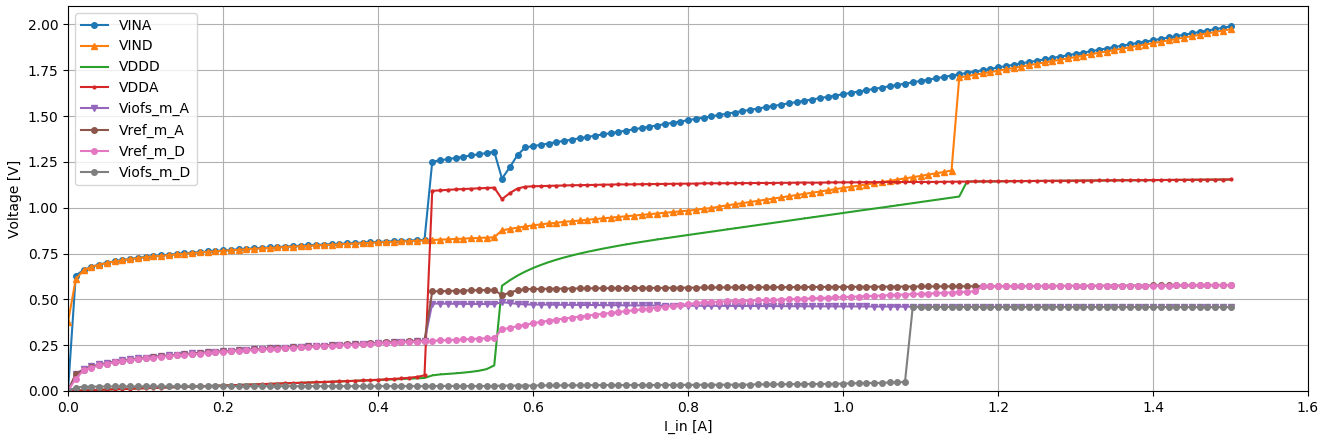
\includegraphics[scale=.3]{Immagini/IUI2}
\caption{Grafico corrente-tensione ottenuto tenendo i due regolatori separati e variando la corrente da 0 A a 1.5 A.}
\label{IUI}
\end{figure}
Le prime misure sono state eseguite utilizzando come riferimento per $\mathrm{V_{out}}$ e $\mathrm{V_{iofs}}$ le tensioni generate internamente al chip. Le misure per i due SLDO, che sono stati tenuti indipendenti, sono state eseguite a livelli di corrente crescenti, partendo da 0 A fino ad arrivare a 1.5 A a passi di 10 mA\footnote{L'incremento di corrente è in contemporanea per i due SLDO.}. 
L'andamento ottenuto è quello riportato in figura \ref{IUI}. L'undershoot ben visibile sulla tensione in ingresso e in uscita della parte analogica è causato da una distribuzione non uguale delle correnti nei due SLDO. 
Quando si attiva la parte digitale si ha un picco di assorbimento di corrente, che causa un drop nella parte analogica:
\begin{center}
\begin{tabular}{ccc }
\hline
$\Delta \mathrm{V_{INA}}$ & $\Delta \mathrm{V_{DDA}}$ &$\Delta \mathrm{V_{DDA}}$  \\ \hline
$\sim$0.150 A & $\sim$ 0.030 A& $\sim$0.060 A\\ \hline     
\end{tabular}
\end{center}

Questo avviene nonostante le alimentazioni dei due SLDO siano separate, in quanto all'interno del chip ci sono zone di 'dialogo' tra regione analogica e digitale. 
La parte digitale si attiva a un valore di $\mathrm{I_{in}}$ di 0.56 A, non riuscendo però ad andare a regime, anche perché la tensione in ingresso non è abbastanza alta da consentire un corretto funzionamento.
Questo è dovuto al ritardo con cui il $\mathrm{V_{iofs}}$ digitale arriva al valore corretto. Come introdotto in precedenza la tensione di riferimento dell'offset è ottenuta dalla caduta di tensione su una resistenza, nel nostro caso di $\sim$250 k$\Omega$, data dal passaggio di una corrente di 2 $\mu$A. Se per vari motivi il circuito che genera questa corrente ha un ritardo nell'accensione questo si ripercuote nell'accensione del chip.  
Se tutti questi problemi sono effettivamente legati all'accensione, dovranno scomparire nel momento in cui lo scan sia eseguito partendo da valori alti di corrente per poi scendere fino a 0 A.

%\begin{center}
%\begin{tabular}{|l|c|c|c|c|}
%\hline
% & \multicolumn{2}{c|}{Digitale} & \multicolumn{2}{c|}{Analogica} \\ \hline
% 
%& media & errore & media & errore \\ \hline
%
%$\mathrm{R_{eq}}$ & 0.752 $\Omega$ & 0.0003 $\Omega$& 0.7178 $\Omega$ & 0.0003 $\Omega$ \\ \hline
%$\mathrm{V_{ofs}}$ & 0.844 V& 0.004 V & 0.9025 V & 0.0003 V\\ \hline     
%
%\end{tabular}
%\end{center}

%\begin{figure}
%\centering
%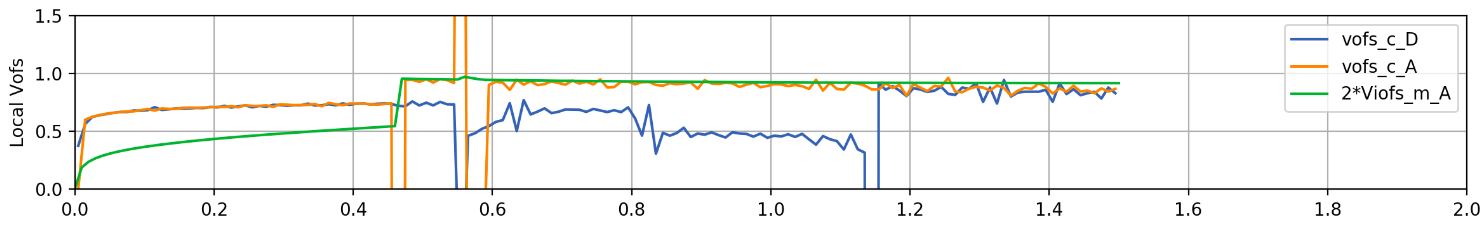
\includegraphics[scale=.27]{Immagini/IUISubPlotVofs}
%\caption{.}
%\label{IUISubPlotVofs}
%\end{figure}

%\begin{center}
%\begin{tabular}{|l|c|c|}
%\hline
%&Digitale  &Analogica \\ \hline
%$\mathrm{R_{eq}}$ & 0.753 $\Omega$& 0.724 $\Omega$ \\ \hline
%$\mathrm{V_{ofs}}$ & 0.845 V & 0.900 V\\ \hline
%\end{tabular}
%\end{center}
\subsubsection{Alimentazioni indipendenti, rampa di corrente decrescente, tensioni di riferimento interne}
\begin{figure}
\centering
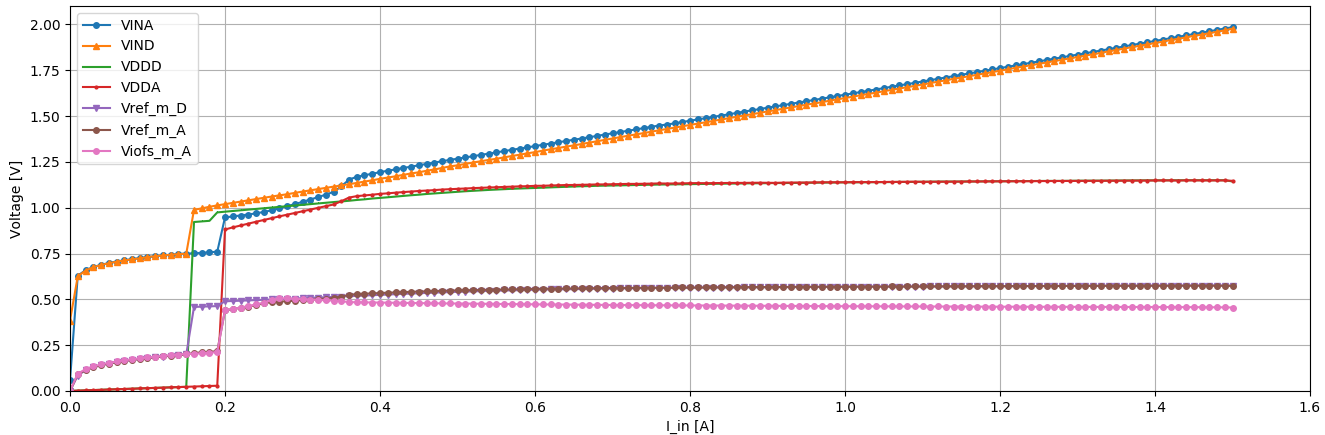
\includegraphics[scale=.3]{Immagini/IDI2}
\caption{Grafico corrente-tensione ottenuto tenendo i due regolatori separati e variando la corrente da 1.5 A a 0 A.}
\label{IDI}
\end{figure}

Una seconda serie di misure, il cui andamento è riportato in figura \ref{IDI}, è stata ottenuta partendo da una corrente in ingresso di 1.5 A e diminuendola fino a 0 A. 
Dal grafico si può notare come gli undershoot presenti nella precedente scansione non siano più visibili, questo è in accordo con la giustificazione data, cioè che siano dovuti all'attivazione del chip, che in questa fase ha consumi più elevati. 
Una volta che il chip ha raggiunto la configurazione di default, i consumi sono di circa 50 mA per la parte digitale e 400 mA per quella analogica. Questo fin tanto che il chip non riceve un segnale di clock esterno. 
Questa differenza in consumi di corrente tra parte analogica e digitale si riflette nel fatto che, diminuendo ulteriormente la corrente, la prima regione ha mostrare problemi è quella analogica, mentre la parte digitale riesce a rimanere attiva anche con correnti inferiori a 200 mA. 
Inoltre, partendo da valori di corrente elevati, e quindi tensioni in ingresso ben al di sopra di quelle minime, non si hanno neppure problemi dovuti a differenti istanti di accensione di parte analogica e digitale.
%\begin{center}
%\begin{tabular}{|l|c|c|c|c|}
%\hline
% & \multicolumn{2}{c|}{Digitale} & \multicolumn{2}{c|}{Analogica} \\ \hline
% 
%& media & errore & media & errore \\ \hline
%
%$\mathrm{R_{eq}}$ & 0.73475 $\Omega$ & 0.00008 $\Omega$& 0.7153 $\Omega$ & 0.0006 $\Omega$ \\ \hline
%$\mathrm{V_{ofs}}$ & 0.86530 V& 0.00007 V & 0.9043 V & 0.0005 V\\ \hline     
%
%\end{tabular}
%\end{center}

Continuando a tenere i due circuiti di alimentazione separati è interessante vedere cosa cambia andando a fornire esternamente le varie tensioni di riferimento.

\subsubsection{Alimentazioni indipendenti, rampa di corrente crescente, $\mathrm{V_{ref}}$ esterna} 
\begin{figure}
\centering
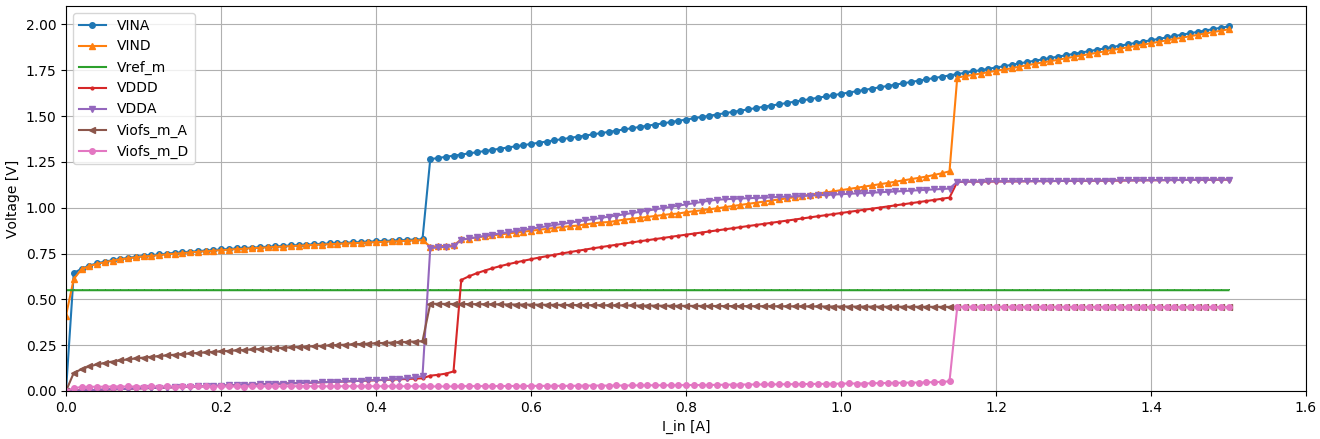
\includegraphics[scale=.3]{Immagini/IUEVref2}
\caption{Grafico corrente-tensione ottenuto tenendo i due regolatori separati e variando la corrente da 0 A a 1.5 A, utilizzando un riferimento esterno per $\mathrm{V_{ref}}=0.550 \V$.}
\label{IUEVref}
\end{figure}
Il grafico riportato in figura \ref{IUEVref} è ottenuto fornendo esternamente  $\mathrm{V_{ref}}=0.550 \V$  sia per la parte analogica che quella digitale. Il comportamento della parte digitale è pressoché analogo a quello ottenuto nel primo grafico \ref{IUI}, mentre per la parte analogica si vede come fornendo $\mathrm{V_{ref}}$ esternamente, non si ha un suo undershoot e dunque non lo si ha nemmeno su $\mathrm{V_{DDA}}$, che però risente ancora del comportamento della parte digitale. Fino a che $\mathrm{V_{iofs\_ m \_ D}}$ non arriva al valore corretto non si ha una situazione stabile (...da riscrivere....).

%\begin{center}
%\begin{tabular}{|l|c|c|c|c|}
%\hline
% & \multicolumn{2}{c|}{Digitale} & \multicolumn{2}{c|}{Analogica} \\ \hline
% 
%& media & errore & media & errore \\ \hline
%
%$\mathrm{R_{eq}}$ & 0.7539 $\Omega$ & 0.00007 $\Omega$& 0.7448 $\Omega$ & 0.0002 $\Omega$ \\ \hline
%$\mathrm{V_{ofs}}$ & 0.84199 V& 0.00011 V & 0.8706 V & 0.0003 V\\ \hline     
%
%\end{tabular}
%\end{center}

\subsubsection{Alimentazioni indipendenti, rampa di corrente crescente, $\mathrm{V_{iofs}}$ esterna} 
\begin{figure}
\centering
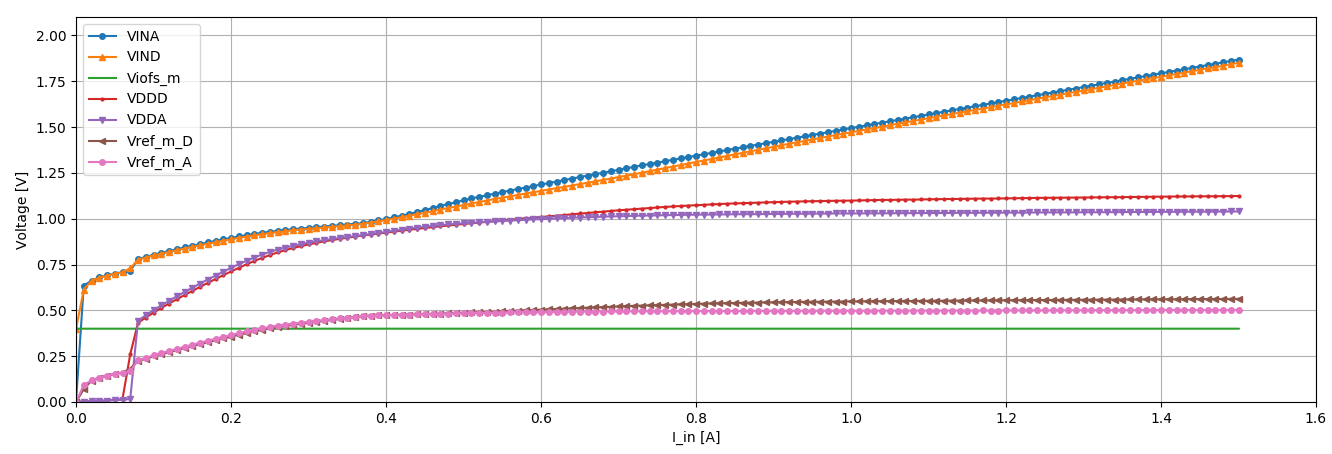
\includegraphics[scale=.3]{Immagini/IUEViofs2}
\caption{Grafico corrente-tensione ottenuto tenendo i due regolatori separati e variando la corrente da 0 A a 1.5 A, utilizzando un riferimento esterno per $\mathrm{V_{iofset}}=0.400 \V$.}
\label{IUEViofs}
\end{figure}
Le stesse misure sono state ripetute fornendo esternamente il solo $\mathrm{V_{iofset}}=0.400 \V$ e quindi utilizzando per $\mathrm{V_{ref}}$ quello interno. In questo caso gli andamenti ottenuti sono decisamente migliori e sono riportati in figura \ref{IUEViofs}. 
Il $\mathrm{V_{iofset}}$ esterno permette di evitare problemi visti in precedenza, quali un differente valore di $\mathrm{I_{in}}$ di attivazione tra parte analogica e digitale.  
%\begin{center}
%\begin{tabular}{|l|c|c|c|c|}
%\hline
% & \multicolumn{2}{c|}{Digitale} & \multicolumn{2}{c|}{Analogica} \\ \hline
% 
%& media & errore & media & errore \\ \hline
%
%$\mathrm{R_{eq}}$ & 0.7871 $\Omega$ & 0.0013 $\Omega$& 0.7554 $\Omega$ & 0.0013 $\Omega$ \\ \hline
%$\mathrm{V_{ofs}}$ & 0.6824 V& 0.0013 V & 0.7403 V & 0.0012 V\\ \hline     
%
%\end{tabular}
%\end{center}

%\begin{figure}
%\centering
%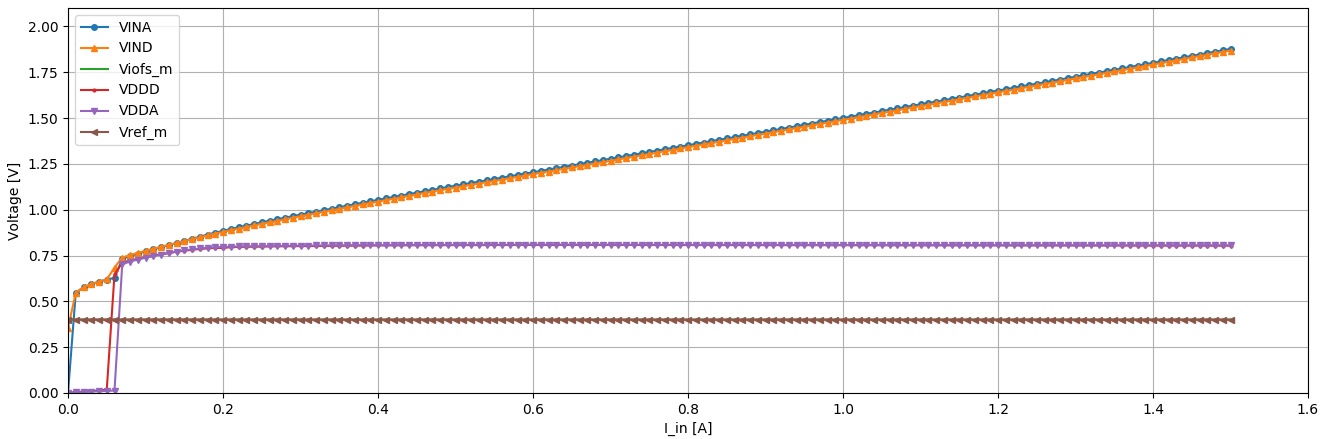
\includegraphics[scale=.3]{Immagini/IUEAll}
%\caption{IUEAll viofs e vref si sovrappongono .}
%\label{IUEAll}
%\end{figure} 
%Infine riportiamo il grafico degli andamenti nal caso in cui sia $\mathrm{V_{ref}}$ che $\mathrm{V_{iofset}}$ sono forniti esternamente. entrambi valgono 0.400, mancanza di kitley

%\begin{center}
%\begin{tabular}{|l|c|c|c|c|}
%\hline
% & \multicolumn{2}{c|}{Digitale} & \multicolumn{2}{c|}{Analogica} \\ \hline
% 
%& media & errore & media & errore \\ \hline
%
%$\mathrm{R_{eq}}$ & 0.7461 $\Omega$ & 0.0004 $\Omega$& 0.7448 $\Omega$ & 0.0004 $\Omega$ \\ \hline
%$\mathrm{V_{ofs}}$ & 0.7452 V& 0.0004 V & 0.7563 V & 0.0004 V\\ \hline 
%\end{tabular}
%\end{center}  

\subsubsection{Alimentazione in parallelo, rampa di corrente crescente, tensioni di riferimento interne} 
\begin{figure}[h]
\centering
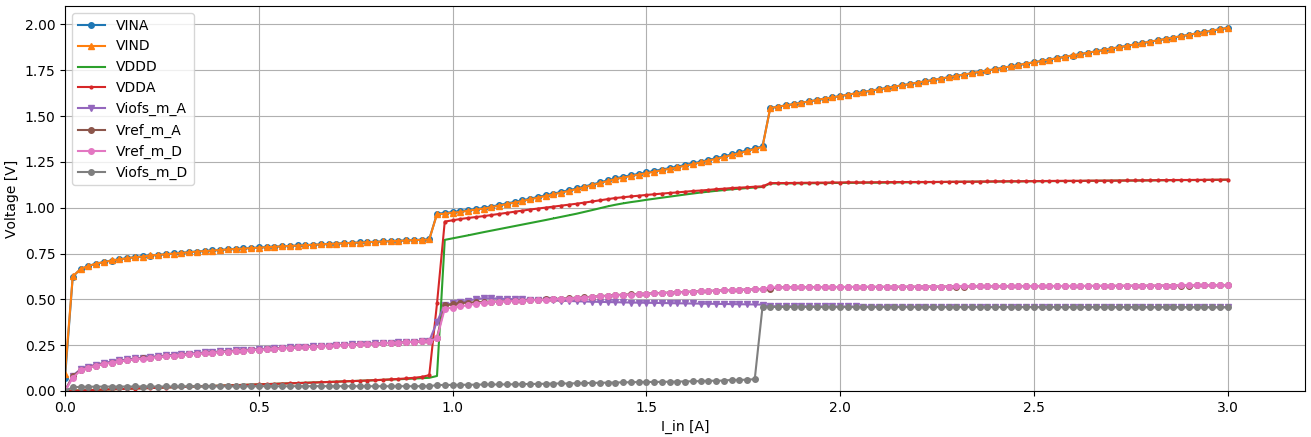
\includegraphics[scale=.3]{Immagini/PUI}
\caption{Grafico corrente-tensione ottenuto con i due regolatori in parallelo e variando la corrente da 0 A a 3.0 A, sull'asse x è riportata la corrente totale che poi si suddivide tra i due regolatori.}
\label{PUI}
\end{figure}
Come detto in precedenza in RD53A è stata lasciata la possibilità di tenere separate le alimentazioni dei due SLDO, nella versione finale i due SLDO si troveranno in parallelo. 
In questa configurazione gli andamenti delle tensioni in ingresso (VINA VIND) e di quelle in uscita (VDDD e VDDA) risultano migliori, come si può vedere dal grafico riportato in figura \ref{PUI}. 
Questo perché la corrente a disposizione per i due Shunt si può suddividere in modo non uguale, fatto che effettivamente accade, lo sbilanciamento nella ripartizioni delle correnti ha inizio quando si 'attiva' $\mathrm{V_{iofs}}$ analogico e termina quando anche $\mathrm{V_{iofs}}$  digitale sale, l'andamento delle correnti è riportato in figura \ref{CurrentSharing}.
%\begin{center}
%\begin{tabular}{|l|c|c|c|c|}
%\hline
% & \multicolumn{2}{c|}{Digitale} & \multicolumn{2}{c|}{Analogica} \\ \hline
% 
%& media & errore & media & errore \\ \hline
%
%$\mathrm{R_{eq}}$ & 0.7441 $\Omega$ & 0.0002 $\Omega$& 0.7396 $\Omega$ & 0.0009 $\Omega$ \\ \hline
%$\mathrm{V_{ofs}}$ & 0.8635 V& 0.003 V & 0.8688 V & 0.0011 V\\ \hline 
%\end{tabular}
%\end{center}

\begin{figure}
\centering
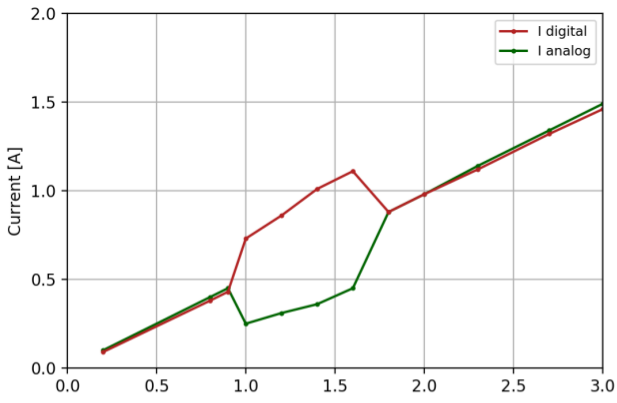
\includegraphics[scale=.4]{Immagini/CurrentSharing}
\caption{Suddivisione della corrente tra i due regolatori posti in parallelo.}%meeting del 16 aprile
\label{CurrentSharing}
\end{figure}
Questo comportamento è stato osservato anche in altri test e riportato in letteratura citazione.. 
Si ha sbilanciamento delle correnti quando  la tensione di uscita di uno dei due regolatori raggiunge la tensione di riferimento, mentre l'altro è ancora al di sotto del livello di riferimento. 
Nel momento in cui i due regolatori raggiungono il valore nominale la distribuzione delle correnti torna ad essere bilanciata. 
Questo comportamento è noto e compreso, il meccanismo che la innesca risiede nell'offset dell'amplificatore A2, che è utilizzato nel current mirror. 
Questo offset porta ad un differente $\mathrm{V_{DS}}$ tra i transistor M1 e M2 che va ad influenzare il rapporto k nella regione lineare. Dunque fin tanto che in uno dei due regolatori la tensione di uscita è minore di quella di riferimento si ha uno sbilaciamento delle correnti. 
Quando viene raggiunto il livello di riferimento M1 e M2 saturano e l'effetto del'offset svanisce.

Questo problema che si verifica durante l'accensione può essere mitigato utilizzando particolari architetture con basso offset per l'amplificatore A2.

Da ognuna di queste configurazioni sono stati ricavati, per la regione in cui il regolatore è attivo, offset e pendenza della curva caratteristica. Ci aspettiamo che la pendenza sia confrontabile con R3 e l'offset con il doppio di $\mathrm{V_{iofs}}$. A questo proposito ricordiamo: 
\begin{center}
\begin{tabular}{lc}
\hline
$\mathrm{R3}$ & 600 $\Omega$ \\%misurata con il multimetro è 620
$\mathrm{V_{iofs}}$ & 0.500 V\\ 
\hline
\end{tabular}
\end{center}

In tabella \ref{table:results} sono riportati i valori di offset e pendenza dell'andamento caratteristico delle tensioni in ingresso per ciascuna configurazione. Riguardo la configurazione è specificato se i due regolatori sono alimentati in parallelo o indipendentemente, se la corrente è stata fatta variare in modo crescente o decrescente e se le tensioni di riferimento per offset e per VDDD e VDDA sono prese internamente o fornite esternamente.

\begin{center}
\begin{table}

\begin{tabular}{|l|c|c|c|c|c|c|c|c|}
\hline
Regolatore & Alim. & Cres./Decr. & \multicolumn{2}{c|}{Vref [V]} & \multicolumn{2}{c|}{Voffset [V]} & Slope [$\Omega$] & Offset [V]\\ \hline
 
Analogico & \multirow{2}{*}{Indip.} & \multirow{2}{*}{Cres.} & Int. & - & Int. & - & 0.7178 & 0.9025 \\
Digitale  &  &  & Int. & - & Int. & - & 0.752  & 0.844 \\ \hline

Analogico & \multirow{2}{*}{Indip.} & \multirow{2}{*}{Decr.} & Int. & - & Int. & - & 0.7153 & 0.9043 \\
Digitale  &  &  & Int. & - & Int. & - & 0.73475  & 0.86530 \\ \hline

Analogico & \multirow{2}{*}{Indip.} & \multirow{2}{*}{Cres.} & Ext. & 0.550 & Int. & - & 0.7448 & 0.8706 \\
Digitale  &  &  & Ext. & 0.550 & Int. & - & 0.7539  & 0.84199 \\ \hline

Analogico & \multirow{2}{*}{Indip.} & \multirow{2}{*}{Cres.} & Int. & - & Ext. & 0.400 & 0.7554 & 0.7403 \\
Digitale  &  &  & Int. & - & Ext. & 0.400 & 0.7871  & 0.6824 \\ \hline

Analogico & \multirow{2}{*}{Paral.} & \multirow{2}{*}{Cres.} & Int. & - & Int. & - & 0.7396 & 0.8688 \\
Digitale  &  &  & Int. & - & Int. & - & 0.7441  & 0.8635 \\ \hline
\end{tabular}
\caption{Risultati ....}
\label{table:results}
\end{table}
\end{center}

errori statistici trascurabili, fluttuazioni dovute a configurazioni 
sempre Requivalente sovrastimata e voff sottostimato
visto anche negli studi del progettista 
per quanto riguarda R3 sembra ci sia in serie una resistenza passiva di circa 0.2 $\Omega$
mentre

\begin{figure}
\centering
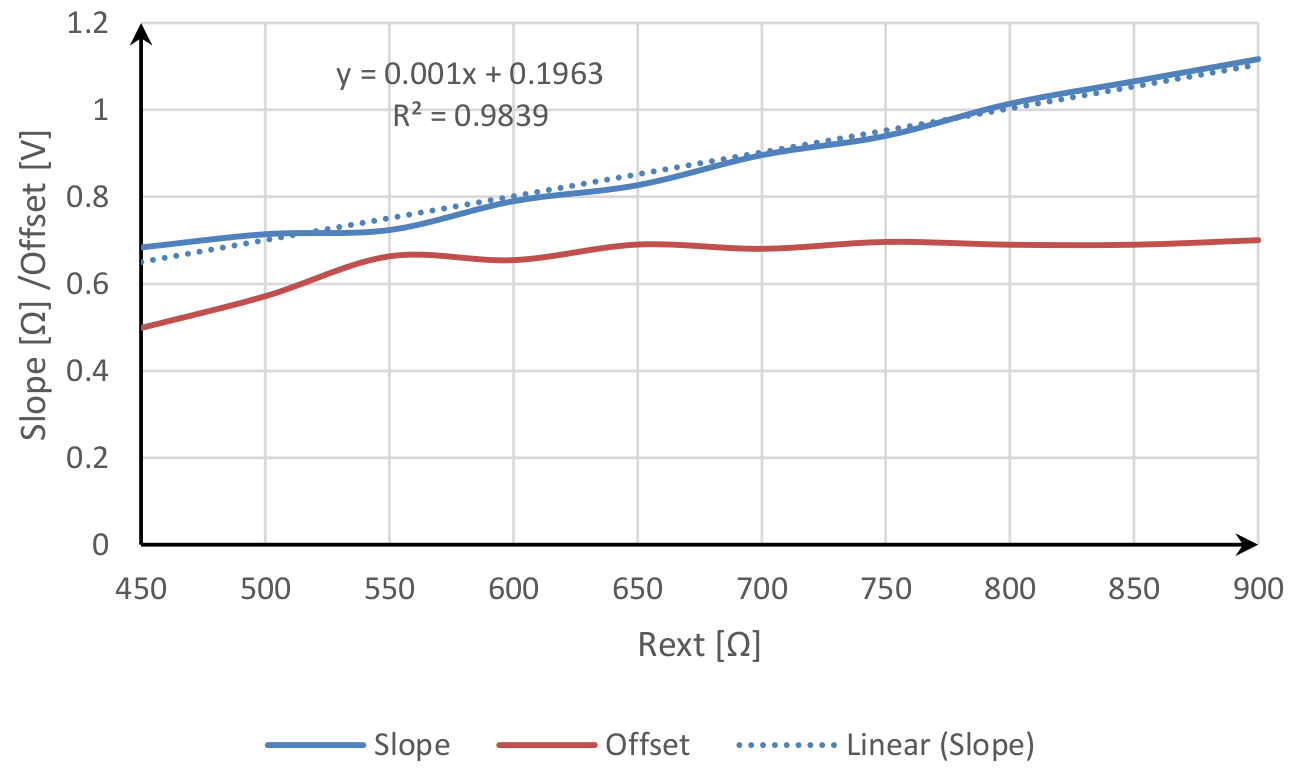
\includegraphics[scale=.3]{Immagini/R3Karagounis}
\caption{ .}%meeting del 13 aprile
\label{R3Karagounis}
\end{figure}

Dal confronto con i valori aspettati risulta evidente che la pendenza della retta caretteristica dello SLDO è sistematicamente maggiore, viceversa l'offset è sistematicamente minore. 
Questo comportamento è stato osservato anche in altri test eseguiti su chip da altri membri all'interno della collaborazione, in particolare sono stati eseguiti test su questo aspetto in modo più approfondito, al fine di comprenderne le cause. 
In figura \ref{R3Karagounis} è riportato l'andamento della pendenza e dell'offset al variare della resistenza R3\footnote{\`E stata utilizzata una resistenza esterna regolabile.}, per interpretare correttamente il grafico ricordiamo che data la presenza nel circuito di un current-mirror con rapporto k = 1000 la pendenza della retta relativa a VIN nel grafico corrente-tensione sarà $\dfrac{R3}{k}$. 
Dal fit lineare risulta che la relazione tra la resistenza esterna e la pendenza è $0.001x + 0.1963$, ciò evidenzia che effettivamente k è 1000, ma vi è una qualche resistenza spuria in serie del valore di circa 0.2 $\Omega$. 
Per quanto riguarda l'offset una sua sottostima è di più difficile interpretazione. 
\begin{figure}
\centering
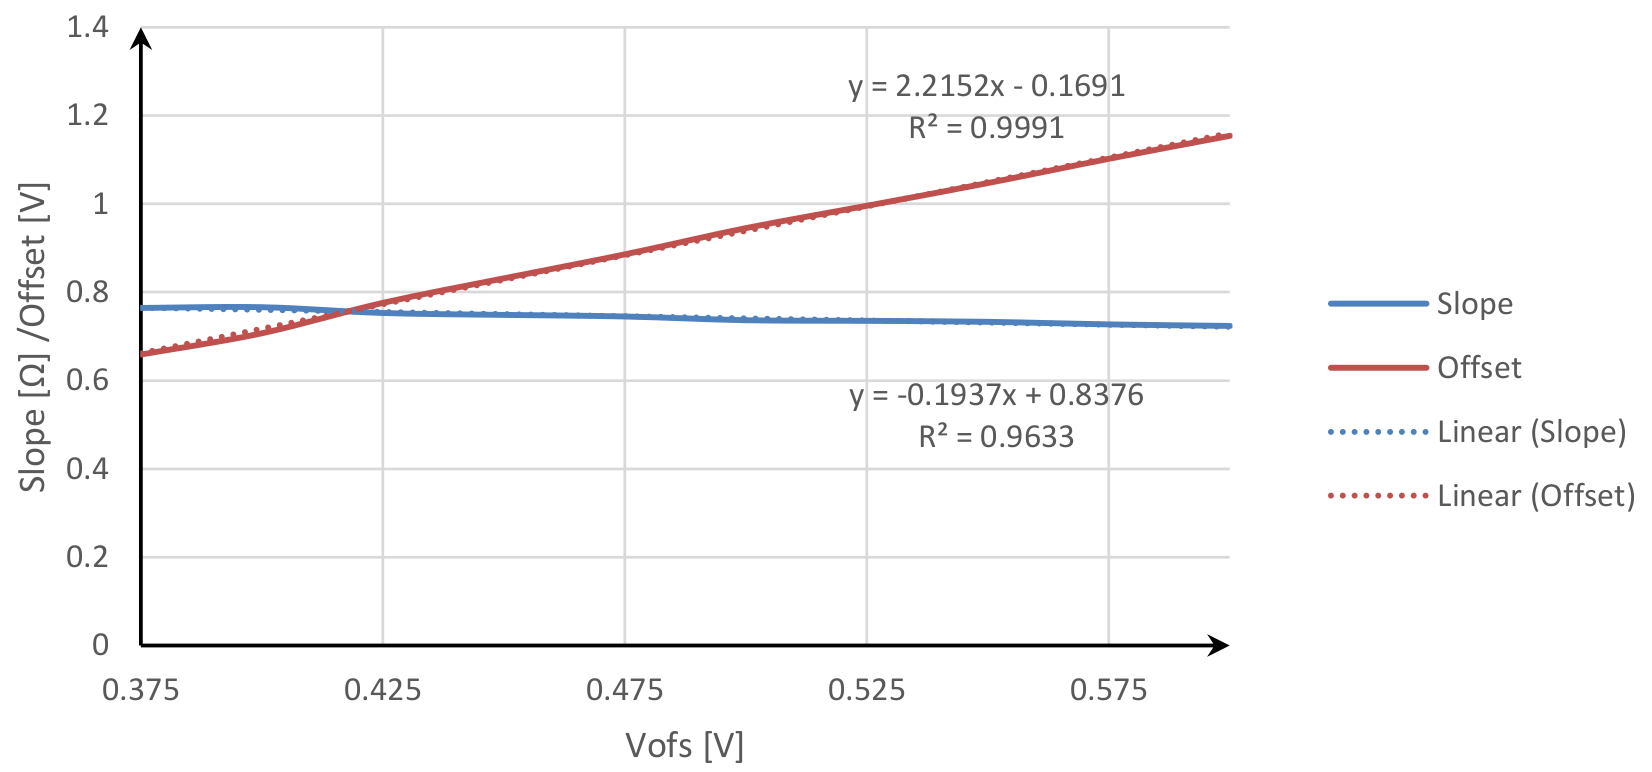
\includegraphics[scale=.25]{Immagini/OffsetKaragounis}
\caption{ .}%meeting del 13 aprile
\label{OffsetKaragounis}
\end{figure}
Anche in questo caso attraverso ulteriori test è stato osservato l'andamento riportato in grafico \ref{OffsetKaragounis} anche perché non dipende solo dal termine noto, ma anche da unfattore moltiplicativo che è maggiore di quello aspettato(2). 
Infine vi è una relazione tra offset e Requivalente, su questo ultimo aspetto sono tutt'ora in corso studi al fine di eliminare questa dipendenza.







\subsection{Variazioni di carico}
Per lo SLDO il carico è rappresentato dal chip, che fino a che si trova nella configurazione di default ha consumi di corrente fissi:
\begin{center}
\begin{tabular}{cc}
\hline
Regione Analogica & Regione Digitale \\ \hline
$\sim$0.400 A & $\sim$ 0.050 A\\ \hline     
\end{tabular}
\end{center}
Le misure riportate di seguito sono invece ottenute andando a variare il carico che è applicato al VDDD/VDDA, questo è stato possibile andando a porre in parallelo al chip un Kitley utilizzato dome sink di corrente... I jumper sulla SCC sono stati posizionati in modo da essere in configurazione SLDO con i due circuiti di alimentazione in parallelo. 
Per queste misure la corrente in ingresso è stata fissata a 2 A, che dunque corrisponde ad 1 A per ciascuno dei due SLDO. 
Dati i diversi consumi tra parte analogica e digitale, l'intervallo in cui è stato fatto variare il carico è stato scelto diversamente. Nel caso in cui il carico sia in parallelo alla parte digitale l'intervallo scelto è tra 0 A e 1 A, mentre nel caso analogico tra 0 A e 0.69 A. 
Queste variazioni di carico non sono dinamiche ma piuttosto vanno considerate come statiche. Infatti tensione di ingresso e di uscita vengono misurate ad ogni incremento del valore del carico. 
Gli andamenti riportati di seguito vanno intesi come una deriva del valore della tensione prodotta dal regolatore. 
Per primo sono riportati gli andamenti ottenuti con il carico applicato alla parte digitale, figura \ref{LoadVDDD}. 
\begin{figure}
\centering
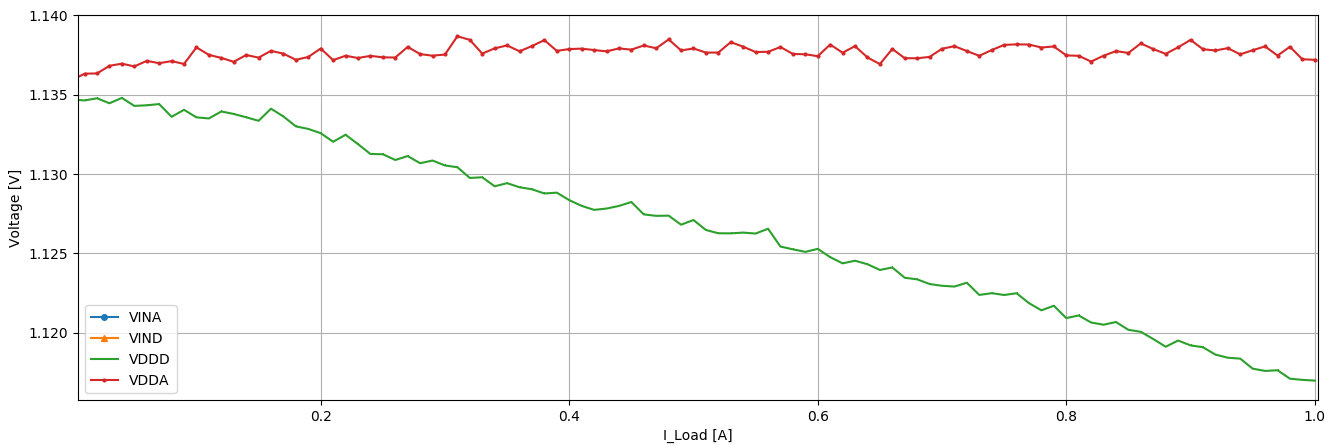
\includegraphics[scale=.3]{Immagini/LoadVDDD}
\caption{LoadVDDD}
\label{LoadVDDD}
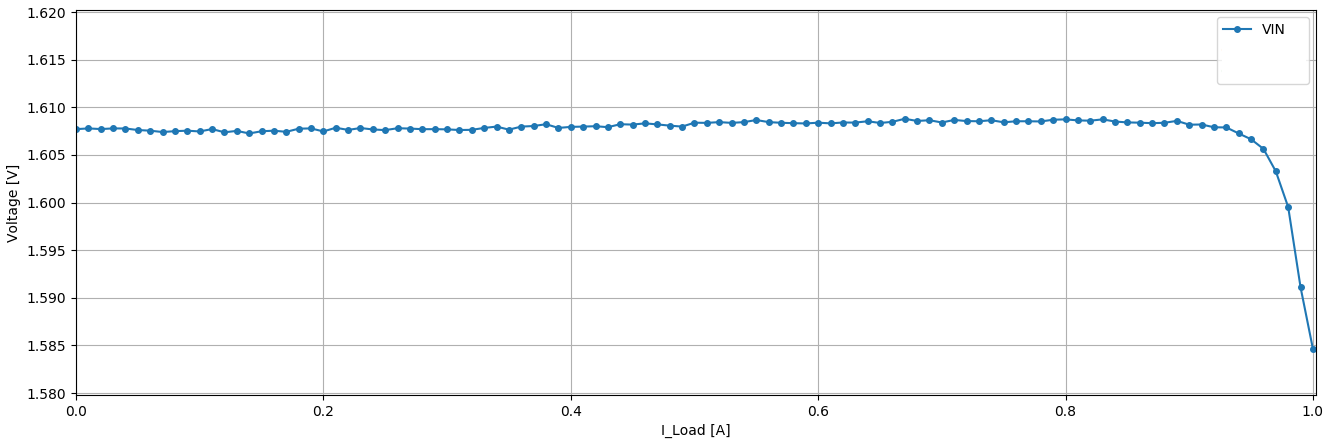
\includegraphics[scale=.3]{Immagini/LoadVIND}
\caption{LoadVIND}
\label{LoadVIND}
\end{figure}
Come si può vedere in grafico \ref{LoadVDDD}, la tensione di alimentazione della regione digitale diminuisce gradualmente arrivando ad una variazione di $\sim$18 mV per un carico addizionale di 1 A, mentre la parte analogica non risente di queste variazioni, restando costante. 
L'andamento della tensione in ingresso, figura \ref{LoadVIND}, ha invece una caduta di $\sim$24 mV che però si concentra nella parte finale partendo circa per valori di carico di 0.940 A, questo comportamento è plausibile se si considera che da sola la parte digitale consuma 50 mA e dunque la somma delle correnti assorbite tre chip e carico supera 1 A, che è quella a disposizione. 
\begin{figure}
\centering
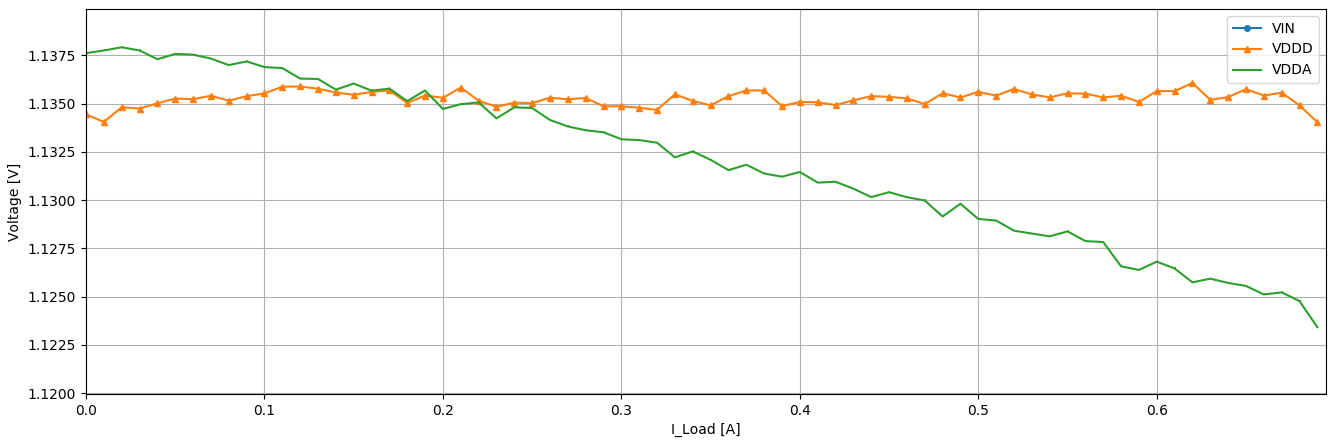
\includegraphics[scale=.3]{Immagini/LoadVDDA}
\caption{LoadVDDA.}
\label{LoadVDDA}
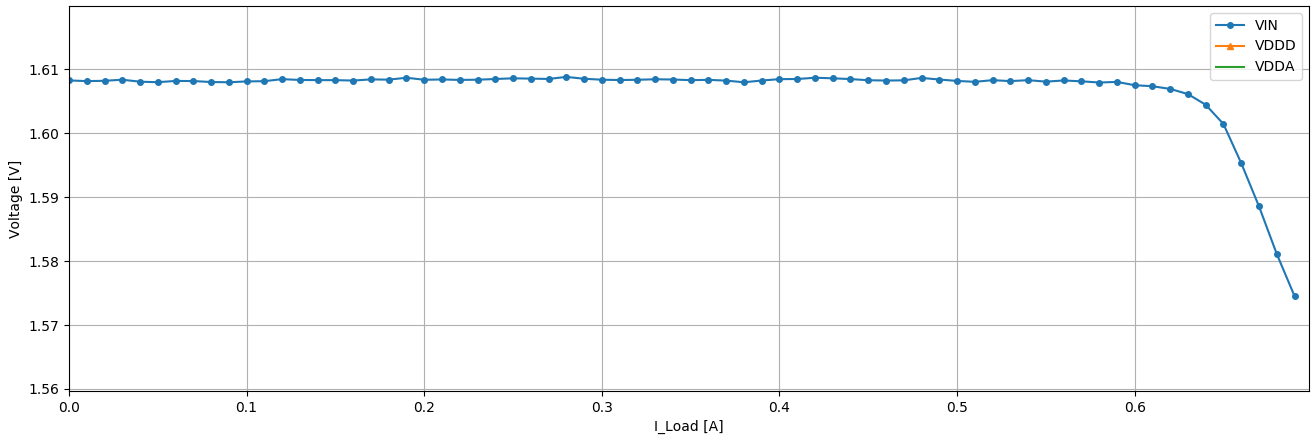
\includegraphics[scale=.3]{Immagini/LoadVINA}
\caption{LoadVINA}
\label{LoadVINA}
\end{figure}
Discorso analogo si può fare per quanto riguarda la parte analogica, in questo caso però i consumi minimi per il chip sono $\sim$400 mA. L'andamento della tensione prodotta dal regolatore è riportata in figura \ref{LoadVDDD}, mentre per quanto riguarda la tensione in ingresso il grafico di riferimento è \ref{LoadVINA}. 
Per la tensione di uscita la caduta è di $\sim$15 mV ed aumenta gradualmente. La tensione in ingresso ha invece una diminuzione di $\sim$26 mV in corrispondenza di un carico di 0.690 A, va ricordato che il consumo totale di corrente in questo caso è al di sopra di 1 A, la diminuzione di tensione ha inizio con un carico di $\sim$0.610 A.

\subsection{Fast ramp-up}
\begin{figure}
\centering
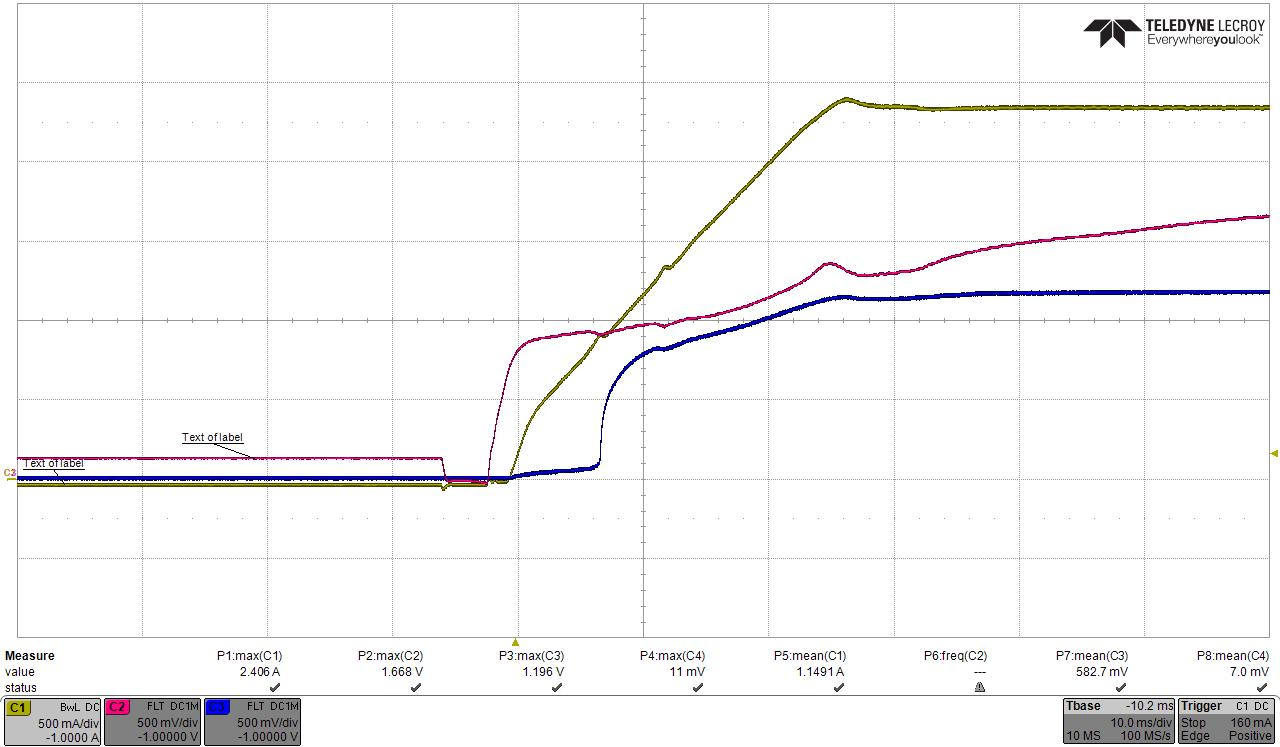
\includegraphics[scale=.3]{Immagini/rd-powup-dir6}
\caption{In giallo è riportata la corrente che in 25 ns passa da 0 A a 2.4 A, in fucsia la tensione in ingresso e in blu la tensione con cui è alimentata la parte digitale del chip VDDD.}
\label{rd-powup-dir6}
\end{figure}

\begin{figure}
\centering
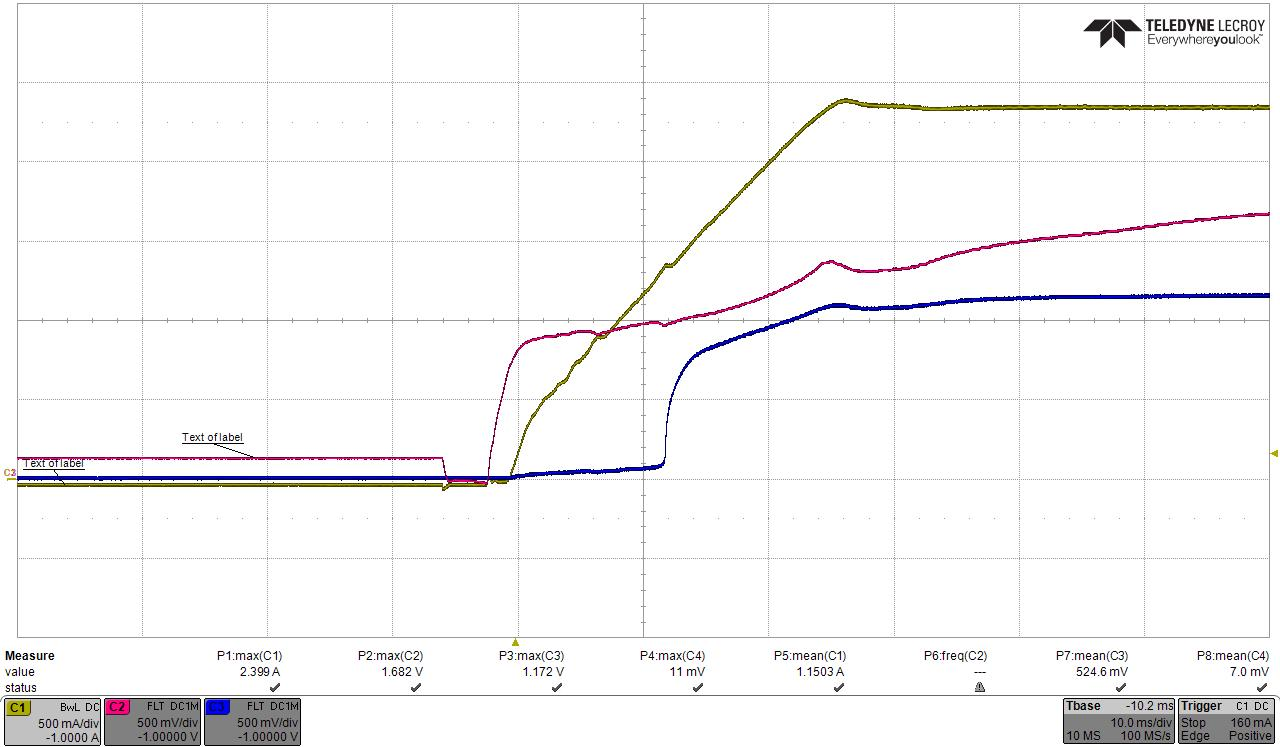
\includegraphics[scale=.3]{Immagini/rd-powup-dir7}
\caption{In giallo è riportata la corrente che in 25 ns passa da 0 A a 2.4 A, in fucsia la tensione in ingresso e in blu la tensione con cui è alimentata la parte analogica del chip VDDA.}
\label{rd-powup-dir7}
\end{figure}
Le misure riportate fino ad ora, per quanto riguarda lo studio dei circuiti di SLDO, sono da considerare statiche, in quanto sono ottenute su tempi scala lunghi in confronto al tempo di risposta dello SLDO. 
%Fino ad ora gli scan sono stati eseguiti lentamente, in confronto al tempo di risposta del circuito di alimentazione, infatti tra un valore di corrente ed il successivo vi è quasi un secondo.
Nel momento in cui il chip sarà collegato ad un sistema di acquisizione dati, il consumo di regione analogica e digitale si modificherà e in base alle operazioni richieste si avranno consumi variabili, che ci aspettiamo il circuito di SLDO sia in grado di gestire. 
In particolare una fase ancor più delicata da questo punto di vista è quella di accensione, in questa fase le variazioni di corrente sono i maggiori. 
Per queste ragioni si è proceduto ad eseguire scansioni in corrente passando da 0 A a 2.4 A in 25 ns con un incremento costante. I due SLDO sono messi in parallelo, quindi si suddividono la corrente erogata dal generatore. Come è possibile vedere dagli screenshoot presi utilizzando l'oscilloscopio non sono presenti oscillazioni durante questa fase di accensione, figura \ref{rd-powup-dir6} e \ref{rd-powup-dir7}. 
Come già visto in precedenza parte digitale e analogica non si attivano nello stesso momento, in particolare VDDD si attiva dopo, questo è in accordo con le misure precedenti.


\section{Sviluppi}
Questi studi sull'alimentazione del chip si collocano in un più ampio progetto di sviluppo del nuovo tracciatore di fase due. In contemporanea a questi viene portato avanti lo sviluppo di sistemi di acquisizione dati in grado di dialogare con il chip e si stanno effettuando test sui tre front end per studiarne la risposta sia prima che dopo processi di irraggiamento. 
In questo situazione lo sviluppo del circuito di alimentazione ha importanti legami con lo sviluppo del resto del chip, come detto il chip ha due regioni alimentate separatamente, digitale e analogica, questa scelta è dettata anche dalla necessità di proteggere la parte analogica, più sensibile, dal rumore della parte digitale. Se l'alimentazione fosse comune il rumore della parte digitale del chip andrebbe ad intaccare la parte analogica che è molto sensibile da questo punto di vista. 
Inoltre per operare una qualsiasi azione a livello di chip è necessario che lo stesso, una volta acceso, si trovi in una configurazione di default ben precisa, la corretta accensione è un problema legato al circuito di ShuntLDO, regione digitale e analogica devono attivarsi correttamente evitando oscillazioni durante il power-up e drop di tensione. 
Risulta quindi chiaro lo stretto legame che vi è tra alimentazione e sviluppo del chip. 

All'interno del lavoro di tesi è stato possibile anche un primo approccio allo sviluppo del sistema di acquisizione, in quanto lo studio riguarda oggetti attualmente in evoluzione essendo prototipi. L'approccio al sistema di DAQ rappresenta naturale in un'ottica di sviluppo del progetto di RD53A. A seguito diamo una breve descrizione del sistema di acquisizione utilizzato e dei primi risultati ottenuti su soglie di lettura e la relativa distribuzione di rumore. 



problemi legati a tensioni di riferimento troppo basse non riesce a dare Phase locked loop non sempre riesce, tensioni di otput troppo basse, causa dei vref bassi per problemi di progettazione dei circuiti di band gap, ma se non fa il pll nonn lo posso configurare a valori più alti.

\section{Sistema di acquisizione dati}
I sistemi di acquisizione dati che attualmente in sviluppo ma che è possibile utilizzare per eseguire alcuni test sono Yarr (Yet Another Rapid Readout) \cite{YARR} e il sistema BDAQ sviluppato dall'Università di Bonn \cite{BDAQ}. 
%immagine sistema di acquisizione
Entrambi i istemi di acquisizione sfruttano fpga programmabili xilinx per il dialogo con il chip. 
Attraverso questi sistemi di acquisizione, sul cui sviluppo e le particolari caratteristiche non ci soffermeremo, non essendo questo il principale obbiettivo di questo lavoro di tesi, è possibile al momento vari test. 
In particolare riferendoci al sistema di acquisizione di Bonn i test più importanti, tra quelli attualmente disponibili, sono:
\begin{itemize}
\item \textbf{scan$\_$digital} This basic scan injects a digital pulse into enabled pixels to test the digital part of the chip.
\item \textbf{scan$\_$analog}  This basic scan injects a specified charge into enabled pixels to test the analog front-end. 
\item \textbf{scan$\_$threshold}  This script scans over different amounts of injected charge to find the effective threshold of the enabled pixels.
\item \textbf{meta$\_$tune$\_$threshold$\_$simple} This meta script simply performs a threshold scan for every possible TDAC to obtainthe optimal value per pixel to get as close to the target threshold as possible. The result is a TDAC mask file.
\end{itemize}
Altro file importante è il file contenente i parametri di configurazione dei registri \textbf{default$\_$chip.yaml}, che ogni volta che uno scan viene lanciato vengono scritti nel chip. 

Attraverso questi test è possibile, anche senza aver collegato un sensore al chip, controllare le funzionalità di parte analogica e digitale separatamente, analizzare la risposta dei tre front end ad un segnale di calibrazione, ricavare una distribuzione delle soglie, la distribuzione del rumore e ottimizzare le soglie localmente (per front end lineare e differenziale). 
A livello di questo lavoro di tesi risulta interessante esaminare il comportamento del circuito di alimentazione mentre il chip dialoga con il sistema di alimentazione così da avere informazioni su cosa accade quando ci sono variazioni nella corrente assorbita, senza dover simulare la cosa esternamente. 
Ad esempio durante il test scan$\_$threshold la parte analogica verifica il livello di soglia di ogni pixel andando a iniettare un segnale via via più grande nel circuito di lettura, in questa situazione è corretto pensare che ci siano variazioni nella corrente assorbita anche grandi. 
Una prima prova che è interessante eseguire consiste nel confrontare una situazione in cui è utilizzato il regolatore con lo Shunt e una situazione in cui non è utilizzato lo Shunt e il chip è alimentato in configurazione LDO. In seguito è lecito chiedersi se, effettivamente in una catena seriale di due chip l'attivita di uno non influenza l'altro. Cioè se il circuito di SLDO riesce ad nascondere al chip eventuali fluttuazioni e rumore  che vi sono nella catena.

\subsubsection{LDOvsSLDO}
Riportiamo di seguito una misura che aiuta a capite quali siano i vantaggi effettivi di utilizzare un circuito di alimentazione che implementi uno Shunt oltre al regolatore. Quello che è stato fatto è monitorare le tensioni di alimentazione del chip, VDDD e VDDA, mentre attraverso il sistema di acquisizione dati veniva richiesto al chip di eseguire il test scan$\_$threshold\footnote{Per cercare di massimizzare gli effetti è stato aumentato il numero di pixel uin cui veniva iniettato contemporaneamente un segnale, anch'esso preso molto grande}. 
In questo modo è stato possibile verificare cosa accade con variazioni di carico prorpie dell'attività del chip, senza doverle simulare esternamente. 
Dal confronto tra i risultati ottenuti in configurazione con o senza shunt è emersa chiaramente l'importanza di questo elemento, non solo per evitare cheun malfunzionamento del chip renda inutilizzabile tutta la catena, ma anche per rendere stabili le tensioni generate dal regolatore. 
\begin{figure}
\centering
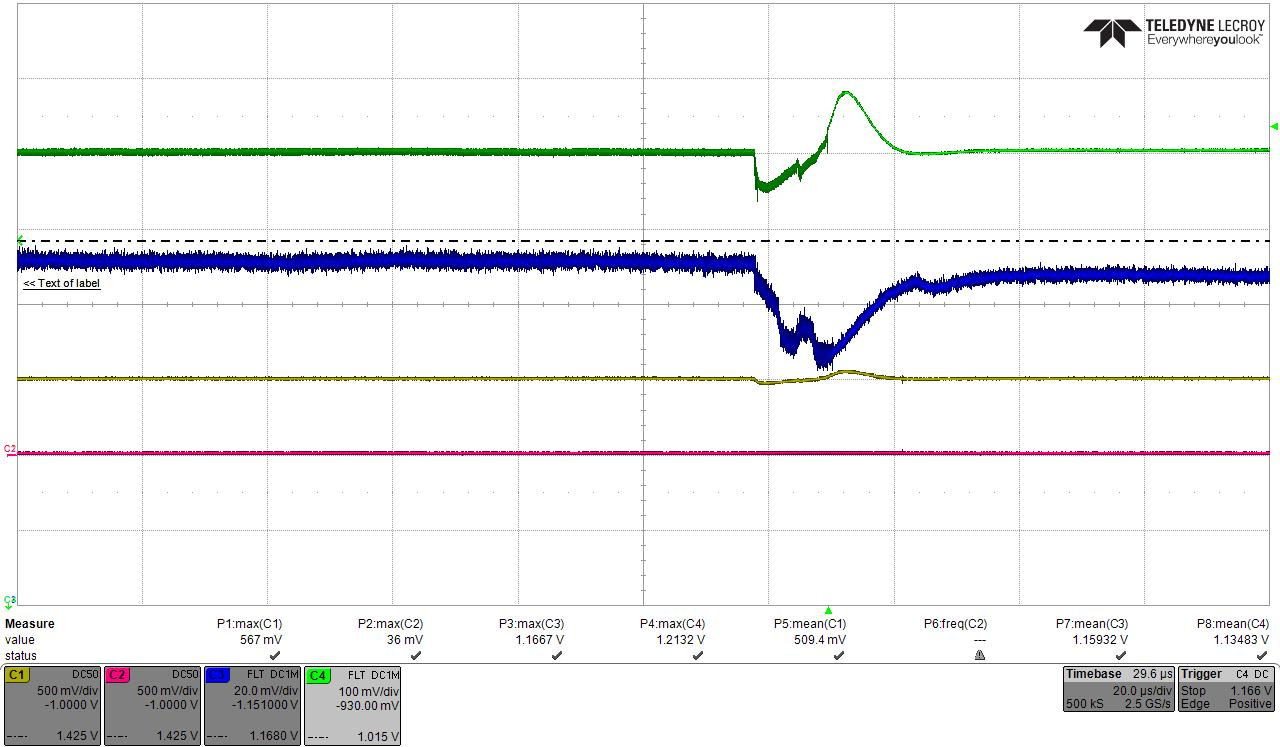
\includegraphics[scale=.3]{Immagini/alllin1}
\caption{VDDD in verde con scala 100 mV/div., e VDDA, in blu con scala 20 mV/div.}
\label{alllin1}
\end{figure}
In figura \ref{alllin1} sono riportate le tensioni VDDD e VDDA in questo caso è stato scelto di utilizzare il chip senza Shunt (alimentato in tensione) e durante il dialogo con il sistema di acquisizione si sono verificate variazioni notevoli nelle tensioni. (per rendere il tutto estremo iniezione di carica su più canali) Con le stessse condizioni utilizzando lo shunt gli sbalzi di tensione sono pressochè spariti (alimentato in corrente), vedi figura \ref{alllin2}, questo perché le variazioni di carico in presenza dello shunt sono gestite localmente, mentre in modalità LDO l'alimentazione è in tensione ed è il generatore esterno che adatta la corrente erogata ai consumi del chip.
\begin{figure}
\centering
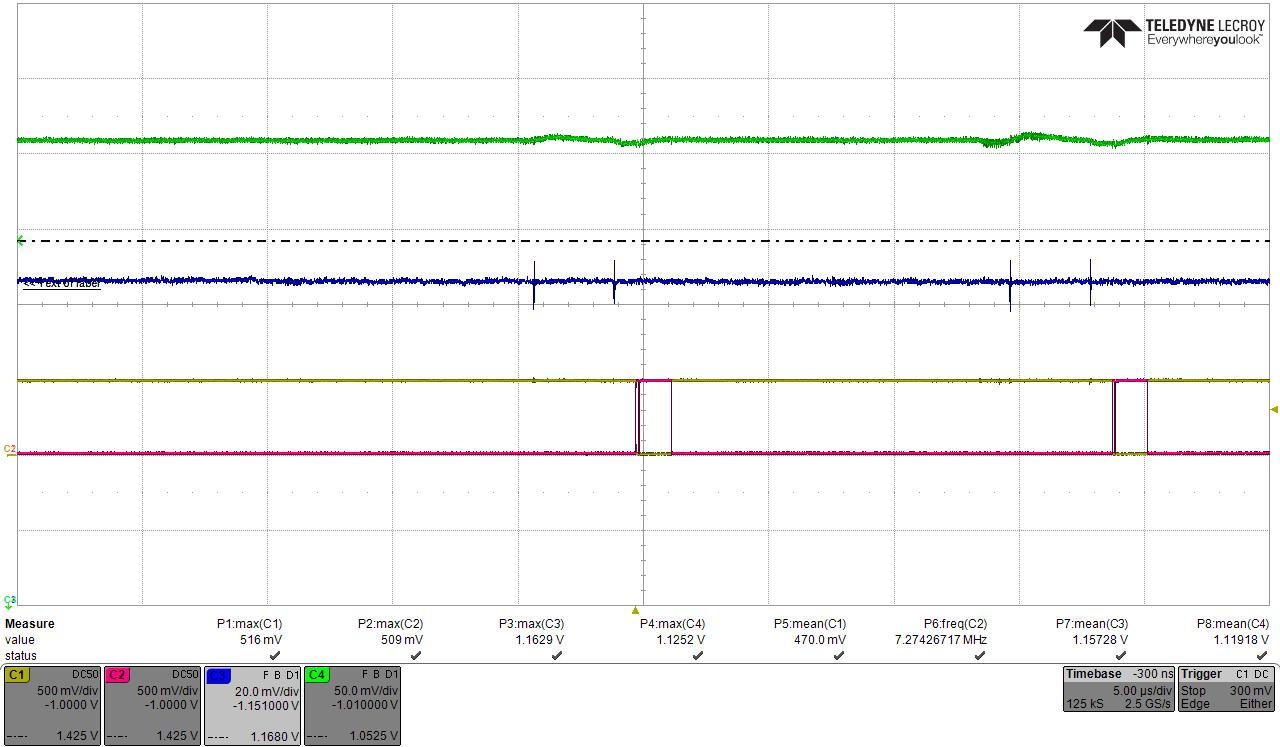
\includegraphics[scale=.3]{Immagini/alllin2}
\caption{VDDD in verde con scala 50 mV/div., e VDDA, in blu con scala 20 mV/div.}
\label{alllin2}
\end{figure}
%\begin{figure}
%\centering
%\includegraphics[scale=.3]{Immagini/}
%\caption{.}
%\label{}
%\end{figure}

\subsubsection{BDAQ}
Prima di procedere con la presentazione dei risultati è necessario dare almento un'idea guida di che operazione vengono eseguite durante lo scan delle soglie al fine di comprendere meglio il significato delle varie distribuzioni.
Attraverso i parametri di configurazione è possibile decidere una soglia globale uguale per tutti i canali di lettura, nella pratica però quello che si otterrà è che la soglia varierà leggermente tra un canale e l'altro. 
Quello che si avrà sarà una distribuzione delle sogglie intorno ad un valore centrale, oltre a questa dispersione delle soglie, a causa del rumore, si avrà che la risposta del circuito di lettura non sarà una theta in funzione della carica raccolta. 
Alle volte il rumore si sommerà al segnale facendo rispondere il discriminatore anche a segnali più piccoli della soglia. Se sul ciascun canale iniettiamo un segnale via via più grande ripetendo il processo più volte e andando a riportare quante volte si ha risposta in funzione del segnale iniettato si ottengono le così dette Scurves, se non ci fosse rumore si avrebbe un gradino. 
Per ogni canale si ha una Scurve messe tutte insieme danno un grafico a "tornado" dove il colore indica quanti sono i pixel che a un dato Vcal si sono accesi un dato numero di volte. Dal fit della singola Scurves si ricava un valore di soglia e rumore, mettendo insieme i risultati per tutti i canali si ottengolo le distribuzioni delle stesse. 
Come detto in precedenza l'utilizzo dello shunt ldo dovrebbe evitare il propagarsi del rumore tra parte analogica e digitale(visto che usano due shuntLDO diversi), ma anche evitare che disturbi della linea vengano visti dal carico. Quello che è stato pensato è mettere due chip in serie alimentati in configurazione SLDO e confrontare la distribuzione di rumore ottenuta in una situazione in cui entrambi i chip effettuano uno scan con la distribuzione ottenuta con un solo chip. 
%immagine setup
\begin{figure}
\centering
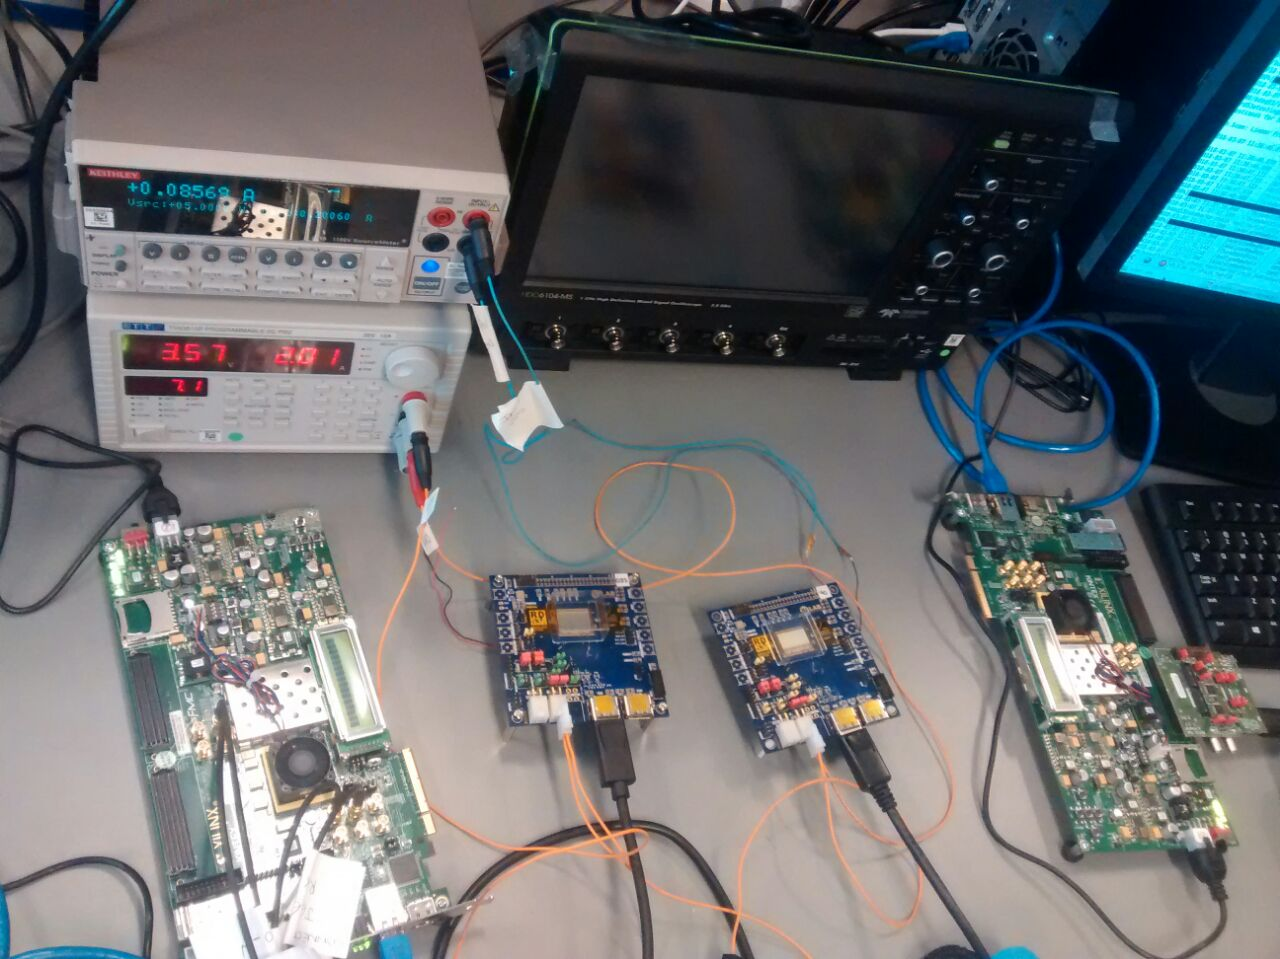
\includegraphics[scale=.2]{Immagini/chipserial}
\caption{.}
\label{chipserial}
\end{figure}
Le misure riportate fanno riferimento solo al front end lineare, in quanto al momento della presa dati era quello su cui era possibile lavorare meglio, sia a livello di ottimizzazione dei vari parametri, sia a livello di software...
I risulati sono riportati in funzione di VCAL, parametro dello scan, la cui conversione in elettroni è 1:10, per una u.a. corrispondono 10 $\mathrm{e^{-}}$.
%immagini distribuzioni
\begin{figure}
\centering
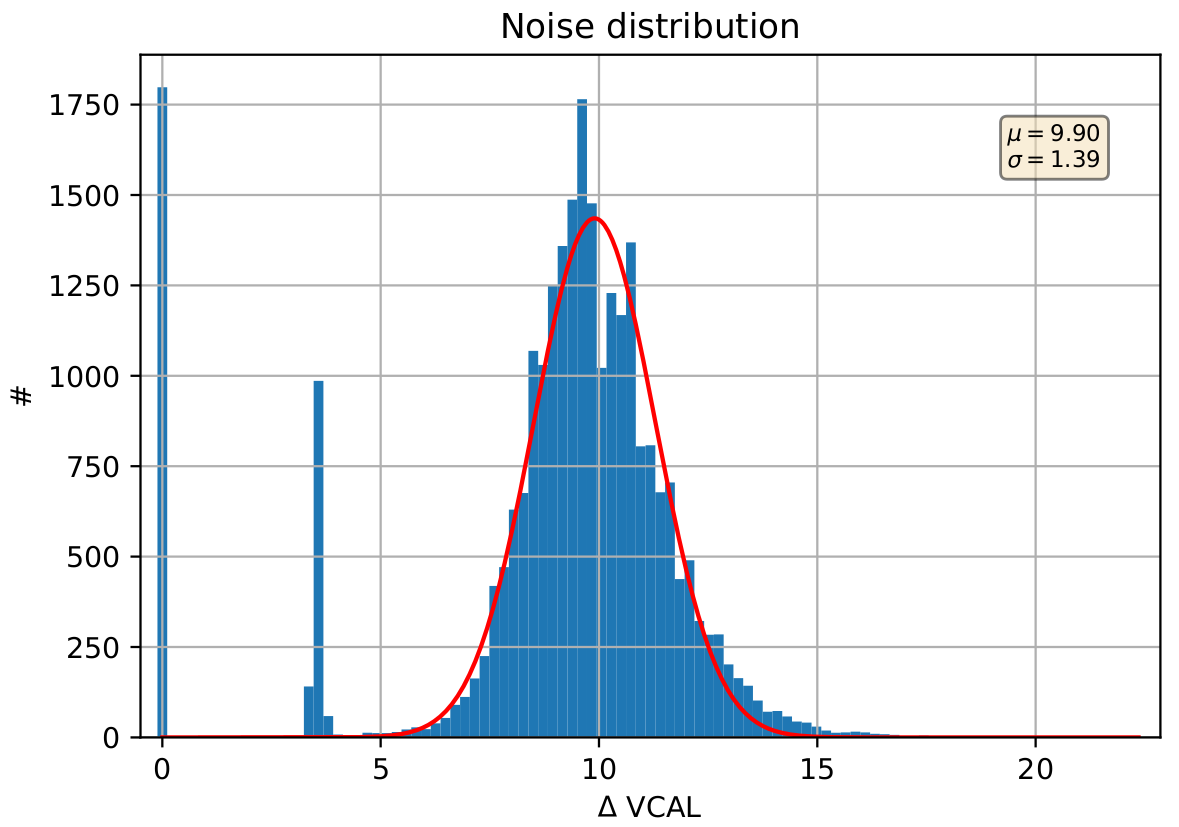
\includegraphics[scale=.3]{Immagini/NoiseSingle}
\caption{noisesingle}
\label{noisesingle}
\end{figure}
come si può vedere dalle due distribuzioni messe a confronto
\begin{figure}
\centering
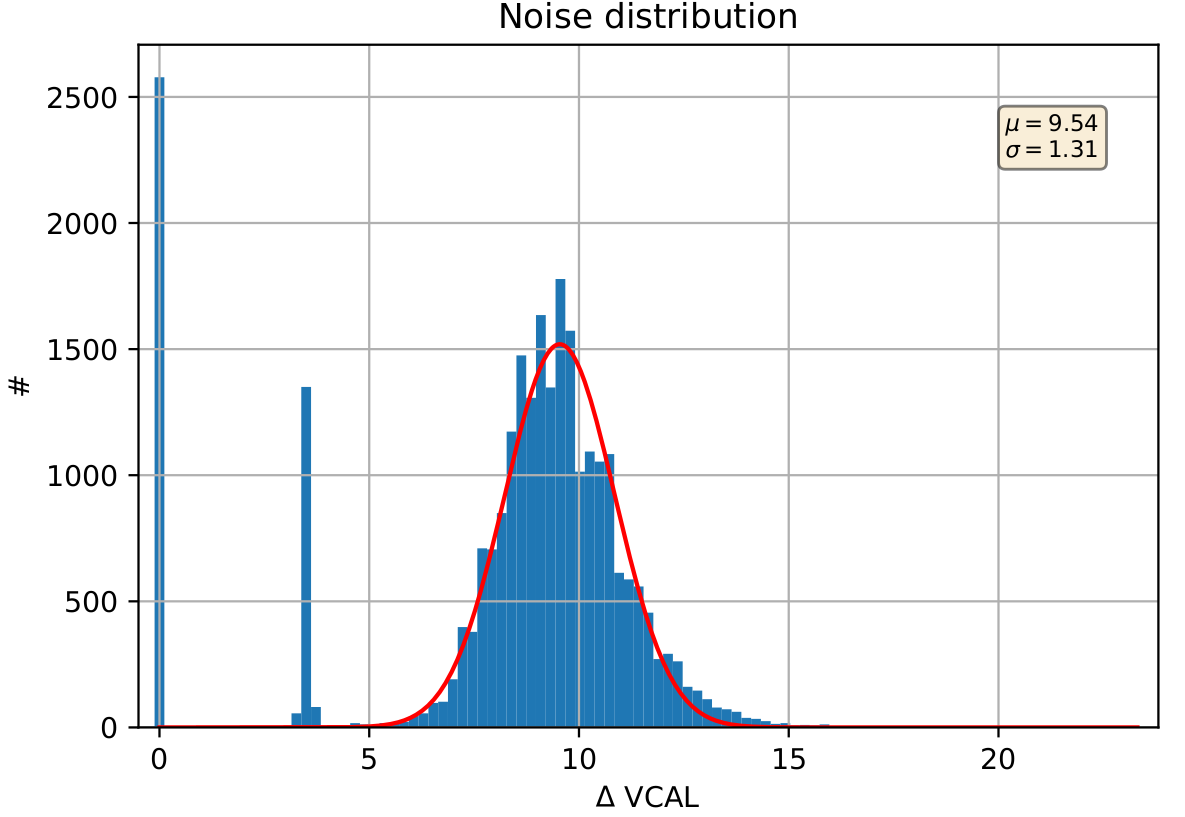
\includegraphics[scale=.3]{Immagini/NoiseSerial}
\caption{noiseserial}
\label{noiseserial}
\end{figure}